\chapter{Analytic Evaluation of the Effective Theory} \label{chap5}

In \chapref{chap4} we introduced the dimensionally reduced effective theory for
heavy quarks at strong coupling. We ended the chapter with a section on the
numerical handling of the theory and its advantages over full lattice gauge
theory simulations. Although a lot of progress has been made evaluating the
predictions of the theory \citep{Fromm:2011qi,Fromm:2012eb,Langelage:2014vpa},
we see from the convergence plots in \figref{fig:numerical_convergence} that
convergence is slow and other approaches should be considered.

It was observed in one of the previous studies of the effective theory
\citep{Langelage:2014vpa} that it is possible to treat the effective theory
purely analytical which provides a plethora of useful methods which we will
explore in this chapter. First and foremost it lends insight into the
mathematical and physical structure of the effective theory and serves as a
cross check for the numerical methods. In \secref{sec:cluster_expansion} we will
present the linked cluster expansion which will provide the building blocks for
a systematic study of the analytic evaluation. We will see how one can translate
between the language of spin statistics and nearest neighbour systems and the
strong coupling, heavy quark formalism. In \secref{sec:analytic_resummation} we
will introduce a new resummation scheme to the analytic evaluation which is
inaccessible to numerical methods. To do this we will exploit the care we put
into the section on effective theory combinatorics.

In \secref{sec:evaluation} we will utilise the full power of the analytic
expressions to study the various aspects of the theory at hand, comparing with
numerical results, studying lattice artefacts and more.

Finally in \secrefs{sec:large_nc_study,sec:yang_lee_zeros} we carry out two
exploratory studies in which the analytic evaluation is paramount. Although
these still pose a lot of open questions, we will build foundations on which
future studies can be performed.

\section{Linked cluster expansion} \label{sec:cluster_expansion}

We start once more on a more fundamental level by introducing the linked cluster
formalism for scalar fields with nearest neighbour interactions. Although the
following section to a sense should be complete, we refer to introductory texts
on the subject for more details, e.g. \citep{Wortis:1980zb,Reisz:1995ag}, and
\citep{Domb:1980zb,Martin:1980zb} for a physics focused presentation of simple
graph theoretical practices. After the fundamentals are out of the way we study
how one can expand the formalism to also include $n$-point interactions with
finite spatial extent, a system in which the effective theory can then be
expressed.

\subsection{Classical linked cluster expansion for nearest neighbour interactions}
\label{sec:classical_lce_nn}

To introduce the framework we consider a scalar field with a $2$-point coupling
%
\begin{equation} \label{eq:scalar_field_Z}
  \mathcal{Z} = \int [\mathrm{d} \phi] e^{-S_0[\phi] + \frac{1}{2} \sum_{x,y}
    \phi(x) v(x,y) \phi(y)},
\end{equation}
%
where function $v(x,y)$ encodes the coupling information.We will assume that the
coupling strength is small enough to justify an expansion around the free
theory. To facilitate the expansion we introduce source fields $J(x)$ and define
the generating functional
%
\begin{equation}
  \mathcal{Z}[J] = \int [\mathrm{d} \phi] e^{-S[\phi] + \sum_x J(x) \phi(x)}.
\end{equation}
%
Since our goal is to study thermodynamic quantities, we shift our attention to
the computation of the grand canonical potential $\mathcal{W}$, or the generating functional
of connected correlation functions
%
\begin{equation}
  \mathcal{W}[J,v] = \log \mathcal{Z}[J,v].
\end{equation}
%
A linked cluster expansion (\emph{LCE}) of the grand canonical potential is then defined as
the Taylor expansion with respect to the coupling $v(x,y)$ around the free
theory
%
\begin{equation} \label{eq:cluster_expansion_def}
  \mathcal{W}[J,v] = \bigg( \exp \bigg(\frac{1}{2} \sum_{x,y} v(x,y)
    \frac{\delta}{\delta \hat{v}(x,y)} \bigg) \bigg) \mathcal{W}[J,\hat{v}]
    \,\Bigg|_{\hat{v}=0}.
\end{equation}
%
One can rewrite the derivative of $\mathcal{W}$ with respect to the couplings in
terms of derivatives with respect to the sources
%
\begin{equation}
  \frac{\delta \mathcal{W}}{\delta v(x,y)} = \frac{\delta^2 \mathcal{W}}{\delta
    J(x) \delta J(y)} + \frac{\delta \mathcal{W}}{\delta J(x)} \frac{\delta \mathcal{W}}{\delta J(y)}.
\end{equation}
%
We also know that $\mathcal{W}[J]$ is the generating functional of the
connected $n$-point functions 
%
\begin{equation}
  \frac{\delta \mathcal{W}}{\delta J(x)} \bigg|_{J=\mathrlap{0}} 
    = \frac{1}{\mathcal{Z}} \int [\mathrm{d} \phi] \, \phi(x) \, e^{-S[\phi]}
    \equiv \langle \phi(x) \rangle,
\end{equation}
%
which for higher order derivatives produces the cumulants
%
\begin{equation}
  \frac{\delta^2 \mathcal{W}}{\delta J(x) \delta J(y)} \bigg|_{J=\mathrlap{0}} 
    = \langle \phi(x) \phi(y) \rangle - \langle \phi(x) \rangle \langle \phi(y) \rangle.
\end{equation}
%
To second order the expansion in \meqref{eq:cluster_expansion_def} is
%
\begin{multline} \label{eq:linked_cluster_2nd_order}
  \mathcal{W}[J, v] = \mathcal{W}[J,0]
    + \frac{1}{2} \sum_{x,y} v(x,y) \frac{\delta \mathcal{W}[J,\hat{v}]}{\delta \hat{v}(x,y)} \bigg|_{\hat{v}=0} \\
    + \frac{1}{8} \sum_{x,y} \sum_{z,w} v(x,y) v(z,w) \frac{\delta^2
      \mathcal{W}[J,\hat{v}]}{\delta \hat{v}(x,y) \delta \hat{v}(z,w)}
    \bigg|_{\hat{v}=0} + \dots
\end{multline}
%
We define the coupled $n$-point functions by
%
\begin{equation}
  \mathcal{M}_n(x_1, x_2, \dots, x_n) = \frac{\delta^n \mathcal{W}[J,v]}{\delta
    J(x_1) \delta J(x_2) \cdots \delta J(x_n)}
\end{equation}
%
which in turn define the free theory $n$-point functions
%
\begin{equation}
   \mathcal{M}_n(x_1, x_2, \dots, x_n) \big|_{v = 0}
   = M_n(x_1) \delta(x_1, x_2, \dots, x_n)
\end{equation}
%
where the Kronecker deltas naturally arise in the free theory
%
\begin{equation}
  x \neq y \hskip .2cm\Rightarrow\hskip .2cm
    \langle \phi(x) \phi(y) \rangle \big|_{v=0} = \langle \phi(x) \rangle \langle \phi(y)
    \rangle.
\end{equation}
%
We can easily see from the deltas that the cluster expansion constitutes an
expansion in connected graphs as everything disconnected would give vanishing
contributions. We can rewrite the second order derivative in $v$ in 
\meqref{eq:linked_cluster_2nd_order} in terms of derivatives w.r.t. the sources,
and thus the free $n$-point functions, which gives
%
\begin{multline} \label{eq:free_energy_before_graph}
  \mathcal{W}[v] = \mathcal{W}[0] + \frac{1}{2} \sum_{x,y} M_1(x) \,v(x,y)\, M_1(y)
  + \frac{1}{4} \sum_{x,y} M_2(x) \,v^2(x,y)\, M_2(y)\\+ \frac{1}{2} \sum_{x,y,z}
  M_1(x) \,v(x,y)\, M_2(y) \,v(y,z)\, M_1(z) + \dots
\end{multline}

\subsection{Graphical definitions}

Although the coefficients for the $v^n$ term can be computed systematically from
\meqref{eq:cluster_expansion_def}  as we showed to second order in
\meqref{eq:linked_cluster_2nd_order}, the process is tedious. However there
exists a formalism in which the terms and their prefactors can be written down
immediately in an intuitive way.
%
%\theoremstyle{definition}%
\begin{definition}{Connected graph}\label{def:graph}\\
  A graph is a set of vertices and bonds where every bond connects two distinct
  vertices. An $n$-rooted graph has $n$ fixed, distinguishable, external
  vertices, while all non-rooted vertices are free. A vertex is said to be
  \emph{$n$-valent} if it has $n$ bonds attached to it.

  A connected graph has the property that one can always move from one vertex to
  another through a continuous set of movements along the graph's bonds. A graph
  which is not connected is disconnected.

  Two $n$-rooted graphs are \emph{isomorphic} if there exists a labelling of the
  bonds and vertices so that the bonds and vertices of the two graphs can be
  made identical. The number of distinct isomorphic labellings of a graph is
  called the graph's \emph{symmetry factor}.
\end{definition}
%
\noindent{}%
To compute $\mathcal{W}$ one simply takes the set of all topologically distinct
$0$-rooted connected graph. The order counting is on the bond level, meaning
that at $\mathcal{O}(v^3)$ we only take $0$-rooted connected graphs with three
or fewer bonds. The final ingredient is a rule for translating between the
graphical representation and the mathematical expression for the grand canonical
potential
%
%\theoremstyle{ruledef}%
\begin{ruledef}{Grand canonical potential $\mathcal{W}$} \label{rule:free_energy}
  \begin{enumerate}
    \item Assign a symbol, $x_1, x_2, \dots, x_n$ to every vertex
    \item To every bond connecting vertices $x_i$ and $x_j$ add a factor
      $v(x_i,x_j)$
    \item For every vertex $x_i$ with valence $p$, add a factor $M_p(x_i)$
    \item Add a sum over the entire lattice for every vertex symbol $x_i$
    \item Divide by the symmetry factor of the graph
  \end{enumerate}
\end{ruledef}
%
\noindent{}%
Using this rule we can write the grand canonical potential in
\meqref{eq:free_energy_before_graph} using a set of graphs
%
\begin{equation}
  \mathcal{W}[v] \:=\:
  \tikz[graph style] \node[skeleton node] {};
  \:+\: \textstyle\frac{1}{2}  \:
  \begin{tikzpicture}[graph style]
    \node[skeleton node] (n1) {};
    \node[skeleton node] (n2) [below=of n1] {};
    \draw[skeleton bond] (n1) -- (n2);
  \end{tikzpicture}
  \:+\: \textstyle\frac{1}{2}  \:
  \begin{tikzpicture}[graph style]
    \node[skeleton node] (n1) {};
    \node[skeleton node] (n2) [position=60 degrees from n1]  {};
    \node[skeleton node] (n3) [position=300 degrees from n2] {};
    \draw[skeleton bond] (n1) -- (n2);
    \draw[skeleton bond] (n2) -- (n3);
  \end{tikzpicture} 
  \:+ \textstyle\frac{1}{4} \:
  \begin{tikzpicture}[graph style]
    \node[skeleton node] (n1) {};
    \node[skeleton node] (n2) [below=of n1] {}
      edge[skeleton bond, bend left=45]  (n1)
      edge[skeleton bond, bend right=45] (n1);
  \end{tikzpicture}
  + \dots \,.
\end{equation}
%
The equality between \ruleref{rule:free_energy} and the grand canonical
potential LCE \meqref{eq:cluster_expansion_def} is in no way trivial and proofs
for the equality are given in e.g.  \citep{Englert:1963pr,Bloch:1965jp}. The
topology of the interaction is still yet to be specified and the sums over the
symbols \{$x_1$,\dots,$x_n$\} run over the entire lattice. Further
simplification can be achieved by choosing e.g. a uniform nearest neighbour
coupling
%
\begin{equation}
  v(x,y) = 
    \begin{cases}
      \hskip .1cm v & \text{ if $x$ and $y$ are nearest neighbours}\\
      \hskip .1cm 0 & \text{ else}.
    \end{cases}
\end{equation}
%
We have chosen nearest neighbour interactions here, although it has been shown
that a graphical expansion non nearest neighbour couplings can be reordered in
such a way that the class of graphs are identical to the nearest neighbour case
\citep{Pordt:1996it}. For nearest neighbour interactions the grand canonical
potential simplifies further
%
\begin{equation} \label{eq:free_energy_with_embedding}
  \mathcal{W}[v] = N M_0 + \frac{q}{2} v N M_1^2 + \frac{q}{4} v^2 N M_2^2
    + \frac{q^2}{2} v^2 N M_1^2 M_2 + \dots
\end{equation}
%
where $q$ is the $2 d$ for a $d$-dimensional square lattice. This factor is
called the embedding number\footnote{Also referred to as the \emph{lattice
    constant} in the lattice community} of a graph onto the lattice, and will
differ from lattice to lattice. For every graph in with a uniform nearest
neighbour interaction the sum over the symbols / coordinates will result in $N$,
the number of lattice sites, times the embedding number of the graph. Although
it might seem wrong to include all possible embeddings as e.g. the $q^2$ in the
$M_1^2 M_2$ term will natually include the embedding corresponding to the
$M_2^2$ term. This is however not a problem as the $M_n$ factors are given in
terms of commutators and applying the methods of moments and cumulants from
\secref{sec:moments_cumulants} we see that the system resolves these issues
automatically. The embedding number is dependent on the lattice, so that e.g.
the three bond graph
%
\begin{equation}
  \begin{tikzpicture}[graph style]
    \node[skeleton node] (n1) {};
    \node[skeleton node] (n2) [right=of n1] {}
      edge[skeleton bond]  (n1);
    \node[skeleton node] [position=60 degrees from n1] {}
      edge[skeleton bond] (n1)
      edge[skeleton bond] (n2);
  \end{tikzpicture}
\end{equation}
%
has an embedding number of zero on a square lattice as there is no way to
resolve the nearest neighbour requirement of \ruleref{rule:free_energy}. On a
triangular lattice on the other hand it would have a non-zero embedding number.
A table of the four bond graphs with symmetry factors and embeddings on a square
lattice can be found in \tabref{tab:graphs_embeddings}. When we later
extrapolate the graphical methods to the effective theory we will see that these
are all graphs needed to carry out a computation to order $\kappa^8$.

\begin{table}[ht]
  \begin{center}
    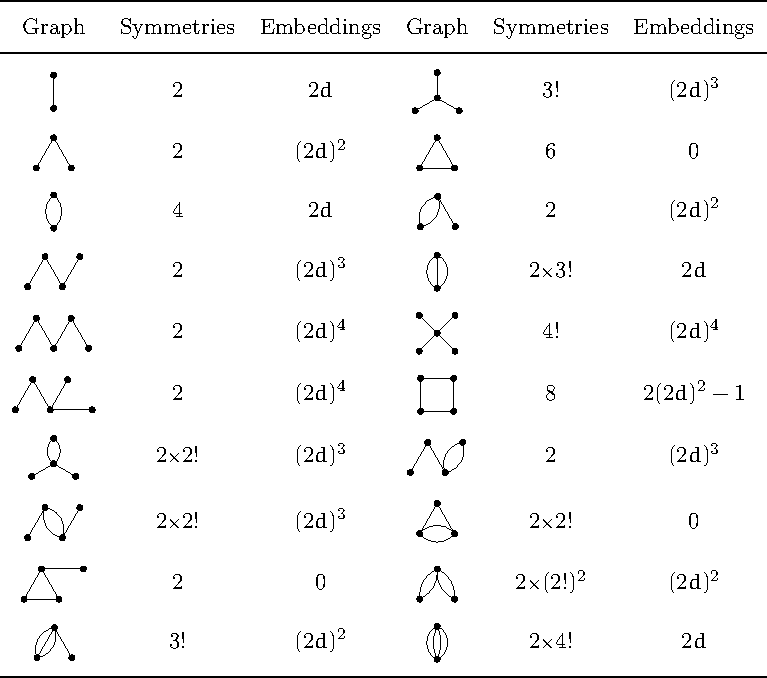
\includegraphics{embedding_and_symmetry}
  \end{center}
  \caption{Graphs with up to four bonds with symmetry factor and the embeddings
  on a $d$ dimensional square lattice.}
  \label{tab:graphs_embeddings}
\end{table}

In the next section we will see how to map the effective theory onto an LCE
framework and the additional condsiderations that has to be taken into account.

\subsection{LCE for the effective theory at LO}

We start working with the leading order action to establish corresponding
quantities in the effective action to the ones introduced in the previous
section. In the dense regime ($\mu \gg T$) the LO effective partition function
is
%
\begin{equation}
  \mathcal{Z}_2 = \int [ \mathrm{d} U ]_0 \det{}^{N_f} \qstat \exp \bigg(-
  h_2 N_f \sum_{\langle x,y \rangle} W_{11} (x) W_{11} (y) \bigg),
\end{equation}
%
as we showed in \chapref{chap4}. Comparing the above equation with the scalar
field partition function we used to introduce the LCE,
\meqref{eq:scalar_field_Z}, we see that there is a close to one-to-one
correspondence between the two systems
%
\begin{equation}
  \phi \Leftrightarrow W_{11}, \hskip .5cm v \Leftrightarrow 2 h_2 N_f, \hskip .5cm
  e^{-S_0[\phi]} \Leftrightarrow \mathcal{J} (U_0, W_{11}) \det \qstat,
\end{equation}
%
where $\mathcal{J} (U_0, W_{11})$ is the Jacobian determinant for the variable
change. There is however no need to compute $S_0[W_{11}]$ explicitly as the free
energy only depends on the $n$-point functions $M_n$, which in turn depends on
expectation values of the free theory. We define the $n$-point functions in
terms of $z$-functions, which are (for $N_f = 1$)
%
\begin{subequations}
\begin{alignat}{99}
  \centermathcell{z_{0}} &= &&\int \mathrm{d} W \det \qstat
    &&= 1 + 4 h_1^3 + h_1^6, \\
  \centermathcell{z_{(11)}} &=  &&\int \mathrm{d} W \det \qstat
    W_{11} &&= 6 h_1^3 + 3 h_1^6, \\
  \centermathcell{z_{(11)^2}} &= &&\int \mathrm{d} W \det
    \qstat W_{11}^2 &&= 4 h_1^3 + 9 h_1^6, \\
  \centermathcell{z_{(11)^3}} &= &&\int \mathrm{d} W \det
    \qstat W_{11}^3 &&= h_1^3 + 17 h_1^6 + h_1^9, \\
  \centermathcell{z_{(11)^4}} &= &&\int \mathrm{d} W \det
    \qstat W_{11}^4 &&= 21 h_1^6 + 6 h_1^9,
\end{alignat}
\end{subequations}
%
while for $N_f = 2$ they take the values
%
\begin{subequations}
\begin{alignat}{99}
  \centermathcell{z_{0}} &= &&\int \mathrm{d} W \det{}^2 \qstat \,
    &&= 1 + 20h_1^3 + 50 h_1^6 + 20 h_1^9 + h_1^{12}, \\
  \centermathcell{z_{(11)}} &=  &&\int \mathrm{d} W \det{}^2 \qstat \,
    W_{11} &&= 15 h_1^3 + 75 h_1^6 + 45 h_1^9 + 3 h_1^{12}, \\
  \centermathcell{z_{(11)^2}} &= &&\int \mathrm{d} W \det{}^2
  \qstat \, W_{11}^2 &&= 6 h_1^3 + 95 h_1^6 + 96 h_1^9 + 9 h_1^{12}, \\
  \centermathcell{z_{(11)^3}} &= &&\int \mathrm{d} W \det{}^2 
  \qstat \, W_{11}^3 &&= h_1^3 + 90 h_1^6 + 188 h_1^9 + 27 h_1^{12}, \\
  \centermathcell{z_{(11)^4}} &= &&\int \mathrm{d} W \det{}^2
  \qstat \, W_{11}^4 &&= 60 h_1^6 + 312 h_1^9 + 81 h_1^{12}.
\end{alignat}
\end{subequations}
%
The $z$'s have a fairly convoluted naming scheme. The reason for this is
that when we include more orders in the effective action we will need to
put sets of $W_{\{nm\}}$ in the integrand. The $z$'s follow the naming scheme
%
\begin{equation} \label{eq:lce_z_definition}
  z_{(n_1 m_1)^{k_1}\cdots(n_p m_p)^{k_p}} = \int \mathrm{d} W \det{}^{N_f} \qstat
  W_{n_1 m_1}^{k_1} \cdots W_{n_p m_p}^{k_p}.
\end{equation}
%
A list of all the integrated $z$'s needed to compute the results we will present
later is given in \apxref{apx:z_functions}. The $n$-point functions are then
given by
%
\begin{subequations}
\begin{align}
  M_0 &= \log z_0, \\
  M_1 &= \frac{z_{(11)}}{z_0}, \\
  M_2 &= \frac{z_{(11)^2}}{z_0} - \frac{z_{(11)}^2}{z_0^2}, \\
  M_3 &= \frac{z_{(11)^3}}{z_0} - 3 \frac{z_{(11)^2} z_{(11)}}{z_0^2} + 2 \frac{z_{(11)}^3}{z_0^3}, \\
  M_4 &= \frac{z_{(11)^4}}{z_0} - 4 \frac{z_{(11)^3} z_{(11)}}{z_0^2} - 3
  \frac{z_{(11)^2}^2}{z_0^2} + 12 \frac{z_{(11)^2} z_{(11)}^2}{z_0^3} - 6 \frac{z_{(11)}^4}{z_0^4}.
\end{align} 
\end{subequations}
%
With the full analytic result for the $\mathcal{Z}_2$ partition function at hand
we can start comparing with results from the numerical evaluation. However,
first we need to establish the observables.


\section{Observables}

We introduced the definition of the observables in \secref{sec:stat-mech}, but
just as we defined them on the lattice in \secref{sec:thermal-lattice-theory},
we have to give them in terms of the parameters we are working with. We use the
fact that  $\mathcal{W}$ is linear in volume in the thermodynamic
limit, which means that the pressure is given simply as
%
\begin{equation}
  \mathcal{P} = T \bigg( \frac{\partial}{\partial V} \log \mathcal{Z}
  \bigg)_{T\mathrlap{,z}} = \frac{T}{V}\,\mathcal{W}.
\end{equation}
%
Similarly, taking the derivative with respect to fugacity is also straight
forward, we can simplify it further using
%
\begin{equation}
  z\, \frac{\partial}{\partial z} \bigg|_{T\mathrlap{,V}} = h_1
  \frac{\partial}{\partial h_1} \bigg|_{T,V}
\end{equation}
%
which means we can define the baryon number density as
%
\begin{equation}
  n_B = \frac{1}{3} n_q = h_1 \frac{1}{3} \bigg( \frac{\partial}{\partial h_1} \frac{\mathcal{W}}{V} \bigg)_{T,V}.
\end{equation}
%
To compute the energy density $e$ we need to compute the
derivative
%
\begin{equation}
  e = T^2 \bigg( \frac{\partial}{\partial T} \frac{\log \mathcal{Z}}{V}
    \bigg)_{z,V}.
\end{equation}
%
We know that $\frac{\log \mathcal{Z}}{V}$ is volume independent, and therefore
the requirement of keeping $V$ constant is automatically fulfilled. We replace
the derivative in $T$ by a derivative in $a$, and therefore have
%
\begin{equation}
  e = -\frac{1}{N_t} \bigg( \frac{\partial}{\partial a} \frac{\mathcal{W}}{V}
    \bigg)_z.
\end{equation}
%
The derivative with respect to the lattice spacing must be handled with a bit of
care. One option is to define the derivative at constant baryon mass
%
\begin{equation}
  a \frac{\partial}{\partial a} (a m_B) = a m_B.
\end{equation}
%
We base the baryon and meson masses on the full heavy quark results from
\citep{Smit:2002introduction}, and later with the additional gauge corrections
from \citep{Langelage:2014vpa}
%
\begin{alignat}{99}
  a m_M &{}={}& \,\acosh &\bigg(1 + \frac{(M^2 - 4)(M^2 - 1)}{2M^2 - 3}\bigg) &&- 24 \kappa^2 \frac{u}{1-u},\\
  a m_B &{}={}& \log &\bigg(\frac{M^3(M^3 - 2)}{M^3 - \frac{5}{4}}\bigg) &&- 18
  \kappa^2 \frac{u}{1-u},
\end{alignat}
%
where $M = \frac{1}{2 \kappa}$. In the strong coupling limit we can use this
to determine $\frac{\partial \kappa}{\partial a}$
%
\begin{multline}
  a \frac{\partial \kappa}{\partial a} = a m_B \Big/
    \:\frac{\partial a m_B}{\partial \kappa} \\
  = \scalemath{0.9}{%
    -\frac{%
        a m_B e^{-a m_B} \big( e^{a m_B} - 8 + 4 \sqrt{4 + e^{a m_B} (e^{a m_B} - 1)} \,\big)%
      }{%
        6 \scalemath{0.8}{\times} 20^{1/3} \sqrt{4 + e^{a m_B} (e^{a m_B} - 1)}
        \big(e^{-a m_B} \big( 2 + e^{a m_B} - \sqrt{4 + e^{a m_B} (e^{a m_B} - 1)} \big) \big)^{2/3}
      }}.
\end{multline}
%
Away from strong coupling one has to define the derivative in $a$ as a
derivative in $\beta$ through the use of implicit functions
%
\begin{equation}
  a \frac{d \beta}{d a} \frac{d \kappa}{d \beta} = - a \frac{d \beta}{d a}
  \frac{\partial a m_B}{\partial \beta} \,\Big/ \:
  \frac{\partial a m_B}{\partial \kappa}.
\end{equation}
%
Assuming strong coupling for now we see that the energy density is given in
terms of the two parameters of the theory
%
\begin{equation} \label{eq:energy_dens_mid_calc}
  e =  -\frac{1}{a N_t} a\frac{\partial \kappa}{\partial a}
    \frac{\partial h_1}{\partial \kappa} \frac{\partial}{\partial h_1}
    \frac{\mathcal{W}}{V} \bigg|_z
  -\frac{1}{a N_t} a\frac{\partial \kappa}{\partial a}
    \frac{\partial h_2}{\partial \kappa} \frac{\partial}{\partial h_2}
    \frac{\mathcal{W}}{V} \bigg|_z.
\end{equation}
%
We use the fact that
%
\begin{equation}
  \frac{\partial h_1}{\partial \kappa} \bigg|_z = \frac{N_t}{\kappa} h_1
\end{equation}
%
to see that the first part of \meqref{eq:energy_dens_mid_calc} is
%
\begin{equation}
  -\frac{1}{a N_t} a\frac{\partial \kappa}{\partial a}
    \frac{\partial h_1}{\partial \kappa} \frac{\partial}{\partial h_1}
    \frac{\mathcal{W}}{V} \bigg|_z
  = - \frac{1}{a} \frac{a}{\kappa} \frac{\partial \kappa}{\partial a} h_1
  \frac{\partial}{\partial h_1} \frac{\mathcal{W}}{V}
  = -3 \frac{1}{a} \frac{a}{\kappa} \frac{\partial \kappa}{\partial a} n_B
\end{equation}
%
after inserting the definition of $n_B$. Using that to first order in $\kappa$
that $\frac{\partial \kappa}{\partial a} \sim \minus{}\kappa \frac{m_B}{3}$ we see that
this first term is somehow related to the rest energy of the system. We subtract
the energy density by this shift, the resulting quantity should give a good estimate for the
binding energy of the system at low temperatures where thermal fluctuations are
suppressed. We define the dimensionless ratio of the binding energy density to
the rest energy to be
%
\begin{equation} \label{eq:epsilon_definition}
  \epsilon = \frac{e - m_{B,\text{eff}}\, n_B}{m_{B,\text{eff}}\, n_B},
\end{equation}
%
where
%
\begin{equation}
  m_{B,\text{eff}} = -3 \frac{1}{\kappa} \frac{\partial \kappa}{\partial a}.
\end{equation}
%
\begin{figure}[t]%
  {\centering%
    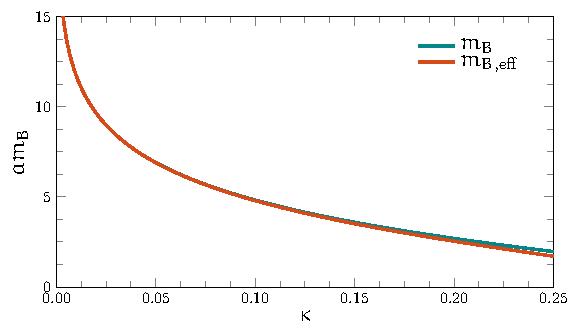
\includegraphics[width=.65\textwidth]{section_2/mb_eff_comparison}\par}
  \caption{Comparison of the effective and full baryon mass used in the definition of $\epsilon$.}%
  \label{fig:mb_eff_comparison}%
\end{figure}%
%
We plot the effective baryon mass vs the real baryon mass in the strong coupling
limit for different values of $\kappa$ in \figref{fig:mb_eff_comparison}, and
see that they mostly agree all the way to $\kappa_{\mathrm{crit}}$, which is far
enough away from the parameter range in this study that the two can be
interchanged.

In \figref{fig:convergence_cluster_Z2} we plot the baryon number density in the
strong coupling limit at varying coupling parameter $h_2$, which can be used to
test the convergence of the expansion, similar to what we did in \chapref{chap4}
with \figref{fig:numerical_convergence} (left). We see that the higher order
linked cluster contribution has a small effect on the convergence, and that it
agrees with the results from the simulations.

\begin{figure}
  \begin{center}
    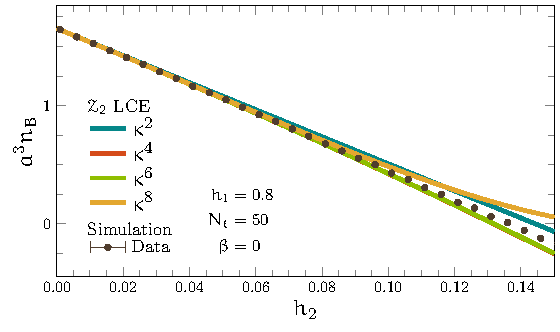
\includegraphics[width=.65\textwidth]{section_2/nb_convergence_cluster_Z2}
  \end{center}
  \caption{Convergence of LCE carried out on the LO effective theory
    $\mathcal{Z}_2$, compared to numerical data for the same parameters.}
  \label{fig:convergence_cluster_Z2}
\end{figure}

\begin{figure}
  \begin{center}
    \begin{adjustbox}{max width=\textwidth}
      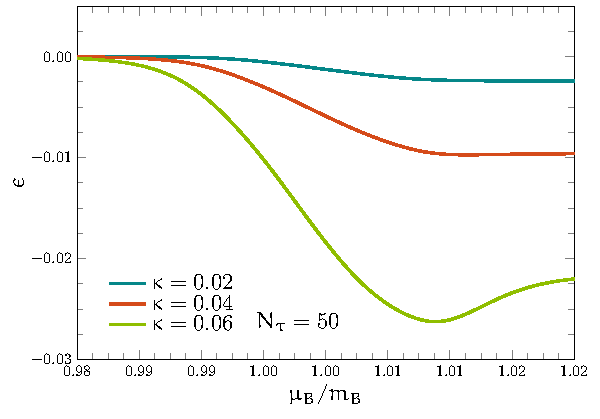
\includegraphics{section_2/binding_energy_Z2_k2}
      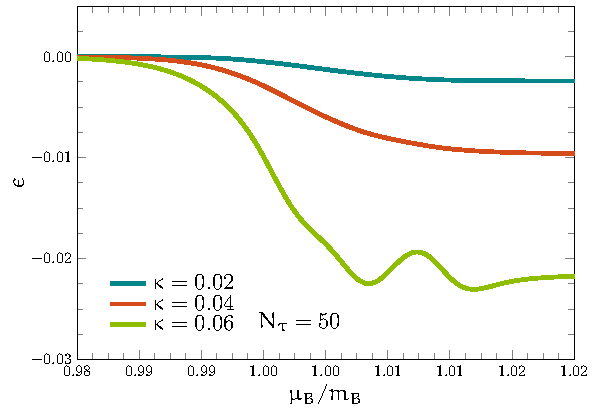
\includegraphics{section_2/binding_energy_Z2_k8}
    \end{adjustbox}
  \end{center} \vskip -.5cm
  \caption{Binding energy $\epsilon$ for three different values of $\kappa$ with
    the $\mathcal{O}(\kappa^2)$ LCE of $\mathcal{Z}_2$ on the left and with the
    $\mathcal{O}(\kappa^8)$ LCE of $\mathcal{Z}_2$ on the right.}
  \label{fig:binding_energy_Z2}
\end{figure}

At this point a note on the multi level expansions is in order. Using the
methods outlined in \chapref{chap4} we compute the effective theory to some
order in the smallness parameters $\kappa$ and $u$. This defines a unique system
with a unique action, which can then be simulated with Monte Carlo or Langevin
algorithms. Another alternative is to analyse the parition function at the given
expansion order and determine the new expansion parameters (in this case $h_2$).
A second expansion can then be carried out to evaluate this specific system
order by order in this expansion parameter. If the simulation converges to the
correct result it is expected to reproduce the full (all order) linked cluster
expansion result of the effective theory at a given order.

Finally we plot the binding energy ratio $\epsilon$ as a function of the
chemical potential for various values of $\kappa$ in
\figref{fig:binding_energy_Z2}. We see that the binding energy decrease the
constituent quark masses (increase $\kappa$), which is what one would expect.
The plot on the left is to leading order in $h_2$, while the plot on the right
shows the fourth order, $h_2^4$, of the expansion. As one can see higher order
solution develops some interesting behaviour at the higher values of $\kappa$ as
we pass the $\mu_B / m_B = 1$ line. It is however beyond convergence, and we
need more orders in the effective theory before we can say anything about the
behaviour at higher chemical potential.

\subsection{Scale setting and the continuum limit}

Up to now we have only considered observables at finite lattice spacing, and
these observables have always been computed as dimensionless ratios of these
so far unspecified lattice spacings. However for us to be able to make any
connections to other fields we first have to determine the physical scale of the
problem. As we outlined in \secref{sec:scale_setting} we need to determine the
scale generated by the regulator, $a$. One way to do this is to analyse the
static potential and link the curvature of this potential to the characteristic
length scale of QCD interactions (the so called \emph{Sommer parameter}
\citep{Sommer:1993ce}). In this way one can determine a function
$a(\beta,\kappa)$ that encodes the scale information. We assume that the heavy
quarks have little influence over the running of the coupling, and therefore for
small $\kappa$ we assume $a(\beta,\kappa) \approx a(\beta)$. We make use of the
interpolation formula for $a(\beta)$ \citep{Necco:2001xg}
%
\begin{multline}
  a = r_0 \exp (-1.6804 - 1.7331(\beta-6) + 0.7849(\beta-6)^2- 0.4428 (\beta-6)^3),\\\text{for } \beta \in [5.7, 6.29],
\end{multline}
%
using the Sommer parameter $r_0 = 0.5 \:\mathrm{fm}$. The interpolation formula
is plotted in \figref{fig:a_of_beta} (left).

\begin{figure}
  \begin{center}
    \begin{adjustbox}{max width=0.99\textwidth}
    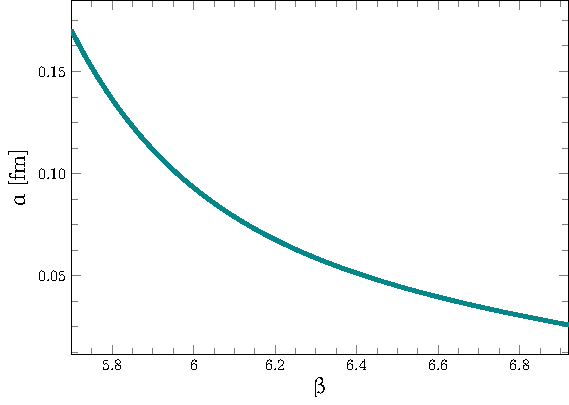
\includegraphics{section_2/a_of_beta_plot}
    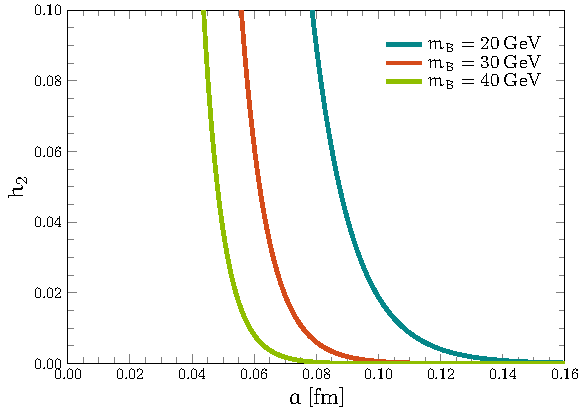
\includegraphics{section_2/h2_of_a_plot}
    \end{adjustbox}
  \end{center}\vskip -.5cm
  \caption{Left: The scale range accessible to the Necco-Sommer interpolation
    formula for strong coupling QCD. Right: The effective nearest neighbour
    coupling $h_2$ as a function of the lattice spacing keeping $m_B$ fixed at
    $T = 10 \:\mathrm{MeV}$.}
  \label{fig:a_of_beta}
\end{figure}

For the continuum limit it is important to vary the variables in such a way that
the physical system remains unchanged. Analogous to how we defined the energy
density by taking the $a$ derivative in such a way that $m_B$ remained constant,
we choose to vary the parameters $\kappa(a), \beta(a), N_t(a)$ in such a way
that $\partial_a m_B = 0$ and $\partial_a T = 0$. Some of the values at
different lattice spacings are shown in \tabref{tab:parameter_values} where we
have fixed the baryon mass to be $30 \: \mathrm{GeV}$. We observe that moving
towards the continuum limit not only decreases the constituent quark masses, but
also increase the number of temporal slices needed to fix temperature. These two
effects combine when computing the effective coupling constant $h_2 = \kappa^2
N_t / N_c$, as is clearly demonstrated in \figref{fig:a_of_beta} (right).

\begin{table}
  \begin{center}
  \begin{tabular}{cccc}
    $\beta$ & $a\hskip .1cm[\mathrm{fm}]$ & $N_t$ & $\kappa$ \\ \toprule
    $5.70$ & $0.170$ & $116$ & $0.000089$ \\
    $5.75$ & $0.152$ & $130$ & $0.000224$ \\
    $5.80$ & $0.136$ & $145$ & $0.000491$ \\
    $5.85$ & $0.123$ & $160$ & $0.000964$ \\
    $5.90$ & $0.112$ & $177$ & $0.001724$ \\
    $5.95$ & $0.102$ & $194$ & $0.002851$ \\ \bottomrule
  \end{tabular} \hskip 1cm
  \begin{tabular}{cccc}
    $\beta$ & $a\hskip .1cm[\mathrm{fm}]$ & $N_t$ & $\kappa$ \\ \toprule
    $6.00$ & $0.093$ & $212$ & $0.004419$ \\
    $6.05$ & $0.086$ & $231$ & $0.006488$ \\
    $6.10$ & $0.077$ & $250$ & $0.009100$ \\
    $6.15$ & $0.073$ & $270$ & $0.012278$ \\
    $6.20$ & $0.068$ & $291$ & $0.016030$ \\
    $6.25$ & $0.063$ & $313$ & $0.020348$ \\ \bottomrule
  \end{tabular} %
  \end{center}
  \caption{Tabulated values of the parameters of interest for the continuum
    study, computed at $T = 10 \:\mathrm{MeV}$ and $m_B = 30 \:\mathrm{GeV}$.}
  \label{tab:parameter_values}
\end{table}

Finally we demonstrate how the continuum limit is approached. We first compute
the desired observable at multiple values for $\beta$, whose upper limit is
determined my the convergence limit of our theory. E.g. the convergence plot
\figref{fig:numerical_convergence} (right) shows us that $h_2 \lesssim 0.04$ for
$\mathcal{Z}_2$ if we require no more than $10 \%$ deviation. If we then fix
$m_B = 30 \:\mathrm{GeV}$ and $T = 10 \:\mathrm{MeV}$ we find an upper limit for
$\beta \lesssim 6.02$. We then analyse the scaling of the observable with
respect to the lattice spacing
%
\begin{equation}
  O_{\mathrm{lattice}} = O_{\mathrm{continuum}} + O_1 \,a + O_2 \,a^2 +
  \mathcal{O}(a^3).
\end{equation}
%
As the expansion is based on unimproved Wilson fermions, the lattice spacing
corrections enter already at the linear level. We somewhat conservatively assume
that we still have $\mathcal{O}(a^2)$ remnants in the observables. We then fit
the observable to this function and extract the continuum limit result from
this. The fit is carried out with two sets of data points, which are chosen
depending on the observable and the value for $\mu$. A common choice here is
$\Delta \beta = 0.01$ and then use the final $10$ and $6$ points respectively
for the two fits. One then averages over the two values and take the difference
as an error estimate for the systematic error. The difference in the observable
at a fixed lattice spacing for two consecutive orders in the expansion is taken
as an error estimate which is included in the fit. The fitting procedure is
illustrated in \figref{fig:continuum_extrapolation} (left). On the right hand
side of the same figure one finds the continuum extrapolated baryon number
density for the $\mathcal{Z}_2$ partition function to the four bond LCE.

\begin{figure}
  \begin{center}
    \begin{adjustbox}{max width=\textwidth}
    \begin{tikzpicture}
      \node[inner sep=0pt] (fig1) {%
        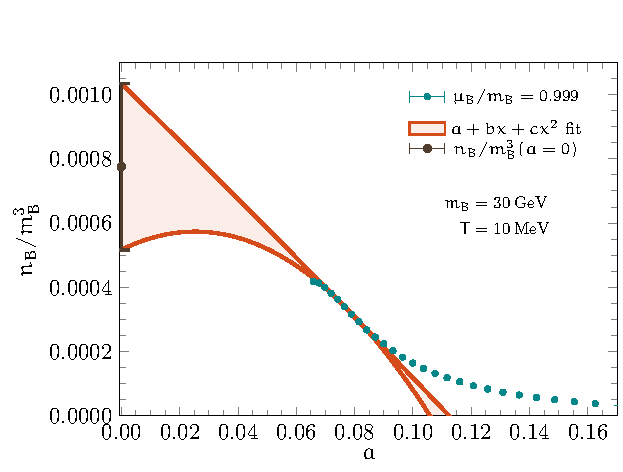
\includegraphics[trim=0 0 0 .95cm, clip]{section_2/nb_of_a_Z2}%
      };
      \node[inner sep=0pt] [right=.2cm of fig1.north east,anchor=north west] {%
        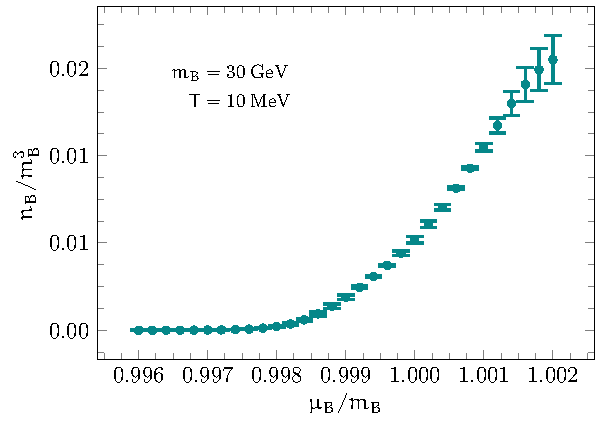
\includegraphics{section_2/nb_continuum_Z2}%
      };
    \end{tikzpicture}
    \end{adjustbox}
  \end{center}\vskip -.6cm
  \caption{Left: Plot demonstrating the continuum limit which is taken at the
    smallest accessible lattice spacing extrapolated with two different data
    sets. Right: The continuum limit of $n_B / m_B^3$ for the LO effective
    theory to four bond LCE.}
  \label{fig:continuum_extrapolation}
\end{figure}

\section{Linked cluster expansion for polymer interactions}

Before we can apply the cluster expansion formalism to the full $\mathcal{O}(u^5
\kappa8)$ effective action we need see how to handle interactions that are more
complicated than two point interactions. In this section we develop a new method
for our tool belt to handle polymer interactions with the linked cluster
formalism. We then establish the necessary mappings and apply it to the higher
order effective theories.

\subsection{Generalisation of the LCE to polymer interactions}

We start with a generalised partition function for $n$ component fields $\phi_i$
%
\begin{multline} \label{eq:multi_point_scalar_Z}
  \mathcal{Z} = \int [\mathrm{d} \phi_i] \exp \bigg(-S_0[\phi_i]
  +\frac{1}{2!} \sum_{x,y} \sum_{i,j} v_{ij}(x,y) \phi_i(x) \phi_j(y) \\
  +\frac{1}{3!} \sum_{x,y,z} \sum_{i,j,k} u_{ijk}(x,y,z) \phi_i(x) \phi_j(y)
  \phi_k(z) + \dots \bigg).
\end{multline}
%
We introduce the sources $J_i$ in a similar fashion to how they were introduced
in \secref{sec:classical_lce_nn}. This gives us a linked cluster expansion for
the grand canonical potential
%
\begin{align}
  \mathcal{W}[v,u] = \bigg[ \exp&\bigg( \frac{1}{2!} \sum_{x,y} \sum_{i,j} v_{ij}(x,y) 
    \frac{\delta}{\delta \tilde{v}_{ij}(x,y)} \bigg)  \nonumber \\
  \times\exp&\bigg( \frac{1}{3!} \sum_{x,y,z} \sum_{i,j,k} u_{ijk}(x,y,z)
    \frac{\delta}{\delta \tilde{u}_{ijk}(x,y,z)} \bigg) \cdots
    \bigg] \mathcal{W}[\tilde{v},\tilde{u}] \Bigg|_{\substack{\tilde{v}=0\\\tilde{u}=0\\\cdots}}\;.
\end{align}
%
The derivative with respect to the 3-point coupling $u$ can be expressed in
terms of derivates w.r.t. the sources
%
\begin{multline}
  \frac{\delta \mathcal{W}}{\delta u_{ijk}(x,y,z)} = \frac{\delta^3 \mathcal{W}}{\delta J_i(x) \delta J_j(y) \delta J_k(z)}
    + \frac{\delta \mathcal{W}}{\delta J_i(x)} \frac{\delta^2 \mathcal{W}}{\delta J_j(y) \delta J_k(z)}
    + \frac{\delta \mathcal{W}}{\delta J_j(y)} \frac{\delta^2 \mathcal{W}}{\delta J_i(x) \delta J_k(z)} \\
  \hspace{2cm} + \frac{\delta \mathcal{W}}{\delta J_k(z)} \frac{\delta^2 \mathcal{W}}{\delta J_i(x) \delta J_j(y)}
    + \frac{\delta \mathcal{W}}{\delta J_i(x)} \frac{\delta \mathcal{W}}{\delta J_j(y)}
    \frac{\delta \mathcal{W}}{\delta J_k(z)}\;,
\end{multline}
%
the same is also true for all the higher $n$-point interactions. To
$\mathcal{O}(v^2, u)$ (two bonds) we get
%
{\allowdisplaybreaks%
\begin{multline} 
  \mathcal{W}[v,u] = \mathcal{W}[0] + \frac{1}{2} \sum M_i(x) \,v_{ij}(x,y)\, M_j(y)
  + \frac{1}{4} \sum M_{ij}(x) \,v_{ik}(x,y)v_{jl}(x,y)\, M_{jl}(y)\\
  + \frac{1}{2} \sum M_i(x) \,v_{ij}(x,y)\, M_{jk}(y) \,v_{kl}(y,z)\, M_1(z)\\
  + \frac{1}{3!} \sum u_{ijk}(x,y,z) M_i(x) M_j(y) M_k(z) \\
  + \frac{1}{2} \sum u_{ijk}(x,y,y) M_i(x) M_{jk}(y) + \dots
\end{multline}}%
%
where the sums have been shortened for the sake of brevity and we have assumed
that the 3-point coupling is cyclic. Just as with the 2-point LCE one can
systematically carry out the lin\}ked cluster expansion, rewriting the derivatives
in the couplings $\{v, u, \dots\}$ order by order and evaluate $\mathcal{W}$.
However a graphical method is desired as it would greatly benefit the
expansion. To do this we need to further specify the geometry of the 3-point
interaction. One natural choice that is compatible with the nearest neighbour
interaction $v$ is a set of two nearest neighbour interactions
%
\begin{equation} \label{eq:udef_wedge}
  u(x,y,z) = 
    \begin{cases}
      \hskip .1cm u & \text{ if $\langle x, y \rangle$ and $\langle y, z \rangle$ are nearest neighbours},\\
      \hskip .1cm u & \text{ if $\langle x, y \rangle$ and $\langle x, z \rangle$ are nearest neighbours},\\
      \hskip .1cm u & \text{ if $\langle x, z \rangle$ and $\langle y, z \rangle$ are nearest neighbours},\\
      \hskip .1cm 0 & \text{ else},
    \end{cases}
\end{equation}
%
where we have reverted to the one-components fields for simplicity. Using this
definition for $u$, $\mathcal{W}$ evaluates to 
%
\begin{multline}
  \mathcal{W}[v,u] = N M_0 + \frac{q}{2} v N M_1^2 + \frac{q}{4} v^2 N M_2^2 \\
    + \frac{q^2}{2} v^2 N M_1^2 M_2 + \frac{q^2}{2} u N M_1^3 + \frac{q}{2} u N
    M_1 M_2 + \dots
\end{multline}
%
Graphically we can represent the above expression as
%
\begin{equation} \label{eq:lce_uv_nn}
  \mathcal{W}[v] \:=\:
  \tikz[graph style] \node[skeleton node] {};
  \:+\: \textstyle\frac{1}{2}  \:
  \begin{tikzpicture}[graph style]
    \node[inner 1] (n1) {};
    \node[inner 1] (n2) [below=of n1] {};
    \draw[bond 1] (n1) -- (n2);
  \end{tikzpicture}
  \:+\: \textstyle\frac{1}{2}  \:
  \begin{tikzpicture}[graph style]
    \node[inner 1] (n1) {};
    \node[inner 1] (n2) [right=of n1]  {};
    \node[inner 1] (n3) [position=60 degrees from n1] {};
    \node[outer 1] (n3o) at (n3) {}
      edge[bond 1] (n1)
      edge[bond 1] (n2);
  \end{tikzpicture} 
  \:+ \textstyle\frac{1}{4} \:
  \begin{tikzpicture}[graph style]
    \node[inner 1] (n1) {};
    \node[outer 1] (n1o) at (n1) {};
    \node[inner 1] (n2) [below=of n1] {};
    \node[outer 1] at (n2) {}
      edge[bond 1, bend left=45]  (n1o)
      edge[bond 1, bend right=45] (n1o);
  \end{tikzpicture}
  \:+\: \textstyle\frac{1}{2}  \:
  \begin{tikzpicture}[graph style]
    \node[inner 2] (n1) {};
    \node[inner 2] (n2) [position=60 degrees from n1]  {};
    \node[inner 2] (n3) [position=300 degrees from n2] {};
    \draw[bond 2] (n1) -- (n2);
    \draw[bond 2] (n2) -- (n3);
  \end{tikzpicture} 
  \:+ \textstyle\frac{1}{2} \:
  \begin{tikzpicture}[graph style]
    \node[inner 2] (n1) {};
    \node[inner 2] (n2) [below=of n1] {};
    \node[outer 2] at (n2) {}
      edge[bond 2, bend left=45]  (n1)
      edge[bond 2, bend right=45] (n1);
  \end{tikzpicture}
  + \dots \,.
\end{equation}
%
Where the $u$ bonds are coloured \ColBaseText{}, the $v$ bond pair is coloured
\ColHlIText{} the nodes are coloured based on the number of fields from which
interaction touches it. This is needed to distinguish e.g. the nodes in the
final term.  An alternative three point coupling could be a triangular nearest
neighbour coupling
%
\begin{equation}
  u(x,y,z) = 
    \begin{cases}
      \hskip .1cm u & \text{ if $\langle x, y \rangle$, $\langle y, z \rangle$,
                      and $\langle x, z \rangle$ are nearest neighbours},\\
      \hskip .1cm 0 & \text{ else},
    \end{cases}
\end{equation}
%
in which case the final term in \meqref{eq:lce_uv_nn} would be excluded as it is
not geometrically realisable. It would actually be better to represent this
particular version of the three point interaction with a three bond diagram
%
\begin{equation}
  \begin{tikzpicture}[graph style]
    \node[inner 2] (n1) {};
    \node[inner 2] (n2) [right=of n1] {}
      edge[bond 2]  (n1);
    \node[inner 2] [position=60 degrees from n1] {}
      edge[bond 2] (n1)
      edge[bond 2] (n2);
  \end{tikzpicture}
\end{equation}
%
as the bonds are intended to encode the nearest neighbour restriction.
Regardless of which geometry the $n$-point interactions have, there are 
numerous paths forward. One option is to compute the derivatives explicitly
order by order and sum over the coordinates explicitly. Alternatively one can
write down all mixed graphs that respect the chosen geometry and compute the
modified symmetry factor. E.g. we see that the two bond nearest neighbour graph
for the $v$ and $u$ interactions
%
\begin{equation}
  \textstyle\frac{1}{4} \:
  \begin{tikzpicture}[graph style]
    \node[inner 1] (n1) {};
    \node[outer 1] (n1o) at (n1) {};
    \node[inner 1] (n2) [below=of n1] {};
    \node[outer 1] at (n2) {}
      edge[bond 1, bend left=45]  (n1o)
      edge[bond 1, bend right=45] (n1o);
  \end{tikzpicture}, \hskip 1cm
  \textstyle\frac{1}{2} \:
  \begin{tikzpicture}[graph style]
    \node[inner 2] (n1) {};
    \node[inner 2] (n2) [below=of n1] {};
    \node[outer 2] at (n2) {}
      edge[bond 2, bend left=45]  (n1)
      edge[bond 2, bend right=45] (n1);
  \end{tikzpicture}
\end{equation}
%
have different symmetry factors due to the fact that the node relabelling
symmetry is broken. A third alternative, and the one we will focus on, is
through a second embedding step
%
\begin{ruledef}{Grand canonical potential $\mathcal{W}$ for $n$ point interactions}%
  \label{rule:free_energy_n_point}%
  \begin{enumerate}
    \item Represent the geometry of the $n$-point interaction $v_n(x_{n_1},
          x_{n_2}, \dots, x_{n_n})$ as a graph according to \defref{def:graph}
    \item Construct all graphs with the necessary number of bonds and geometry
      to the desired order, we refer to these as \emph{skeleton graphs}
    \item Embed all $n$-point interaction graphs onto the skeleton graphs
    \item For every embedded $n$-point graph that visits $x_{n_1}, x_{n_2},
      \dots, x_{n_n}$, add a factor\\ $v_n(x_{n_1}, x_{n_2}, \dots, x_{n_n})$
    \item For every vertex that with \emph{modified valence}\footnote{%
        Modified valence is the number of bonds connecting a vertex originating
        from \emph{different} $n$-point interactions} $p$, add a factor $M_p(x_i)$
    \item The correct symmetry factor will be the symmetry factor of the skeleton
          graph times the number of unique isomorphic embeddings 
  \end{enumerate}%
\end{ruledef}
%
\noindent{}%
Let us consider the embedding of a $v$-link and a $u$-"wedge" from \meqref{eq:udef_wedge}
on the three bond graph
%
\begin{equation}
  \textstyle\frac{1}{2} \:
  \begin{tikzpicture}[graph style]
    \node[skeleton node] (n1) {};
    \node[skeleton node] (n2) [position=60 degrees from n1] {}
      edge[skeleton bond, bend left=45]  (n1) 
      edge[skeleton bond, bend right=45] (n1);
    \node[skeleton node] [position=300 degrees from n2] {}
      edge[skeleton bond] (n2);
  \end{tikzpicture}
\end{equation}
%
This can be done in four different ways
%
\begin{equation}
  \textstyle\frac{1}{2} \:
  \begin{tikzpicture}[graph style]
    \node[inner 1] (n1) {};
    \node[outer 2] (n1o) at (n1) {};
    \node[inner 1] (n2) [position=60 degrees from n1] {};
    \node[outer 2] (n2o) at (n2) {}
      edge[bond 1, bend left=45]  (n1o) 
      edge[bond 2, bend right=45] (n1o);
    \node[inner 2] [position=300 degrees from n2] {}
      edge[bond 2] (n2o);
  \end{tikzpicture}
  +\textstyle\frac{1}{2} \:
  \begin{tikzpicture}[graph style]
    \node[inner 1] (n1) {};
    \node[outer 2] (n1o) at (n1) {};
    \node[inner 1] (n2) [position=60 degrees from n1] {};
    \node[outer 2] (n2o) at (n2) {}
      edge[bond 2, bend left=45]  (n1o) 
      edge[bond 1, bend right=45] (n1o);
    \node[inner 2] [position=300 degrees from n2] {}
      edge[bond 2] (n2o);
  \end{tikzpicture}
  +\textstyle\frac{1}{2} \:
  \begin{tikzpicture}[graph style]
    \node[inner 2] (n1) {};
    \node[outer 2] (n1o) at (n1) {};
    \node[inner 1] (n2) [position=60 degrees from n1] {};
    \node[outer 2] (n2o) at (n2) {}
      edge[bond 2, bend left=45]  (n1o) 
      edge[bond 2, bend right=45] (n1o);
    \node[inner 1] [position=300 degrees from n2] {}
      edge[bond 1] (n2o);
  \end{tikzpicture}
  +\textstyle\frac{1}{2} \:
  \begin{tikzpicture}[graph style]
    \node[inner 2] (n1) {};
    \node[inner 1] (n2) [position=60 degrees from n1] {};
    \node[outer 2] (n2o) at (n2) {};
    \node[outerouter 2] (n2oo) at (n2) {}
      edge[bond 2, bend left=45]  (n1) 
      edge[bond 2, bend right=45] (n1);
    \node[inner 1] [position=300 degrees from n2] {}
      edge[bond 1] (n2oo);
  \end{tikzpicture}
\end{equation}
%
where the first two are isomorphic and can be collected to one term. Hence there
are three unique embeddings of this combination onto the skeleton graph in
question, where one of the embeddings has a non-unit embedding number, and thus
a modified symmetry factor. With these two ingredients we present the
full three bond free energy
%
%\begin{multline} \label{eq:lce_uv_3b}
  \mathcal{W}[v] \:=\:
  \tikz[graph style] \node[skeleton node] {};
  \:+\: \textstyle\frac{1}{2}  \:
  \begin{tikzpicture}[graph style]
    \node[inner 1] (n1) {};
    \node[inner 1] (n2) [below=of n1] {};
    \draw[bond 1] (n1) -- (n2);
  \end{tikzpicture}
  \:+\: \textstyle\frac{1}{2}  \:
  \begin{tikzpicture}[graph style]
    \node[inner 1] (n1) {};
    \node[inner 1] (n2) [right=of n1]  {};
    \node[inner 1] (n3) [position=60 degrees from n1] {};
    \node[outer 1] (n3o) at (n3) {}
      edge[bond 1] (n1)
      edge[bond 1] (n2);
  \end{tikzpicture} 
  \:+ \textstyle\frac{1}{4} \:
  \begin{tikzpicture}[graph style]
    \node[inner 1] (n1) {};
    \node[outer 1] (n1o) at (n1) {};
    \node[inner 1] (n2) [below=of n1] {};
    \node[outer 1] at (n2) {}
      edge[bond 1, bend left=45]  (n1o)
      edge[bond 1, bend right=45] (n1o);
  \end{tikzpicture}
  \:+\: \textstyle\frac{1}{2}  \:
  \begin{tikzpicture}[graph style]
    \node[inner 2] (n1) {};
    \node[inner 2] (n2) [position=60 degrees from n1]  {};
    \node[inner 2] (n3) [position=300 degrees from n2] {};
    \draw[bond 2] (n1) -- (n2);
    \draw[bond 2] (n2) -- (n3);
  \end{tikzpicture} 
  \:+ \textstyle\frac{1}{2} \:
  \begin{tikzpicture}[graph style]
    \node[inner 2] (n1) {};
    \node[inner 2] (n2) [below=of n1] {};
    \node[outer 2] at (n2) {}
      edge[bond 2, bend left=45]  (n1)
      edge[bond 2, bend right=45] (n1);
  \end{tikzpicture}
  \:+ \textstyle\frac{1}{3!} \:
  \begin{tikzpicture}[graph style,node distance=.4]
    \node[inner 1] (n1) {};
    \node[outer 1] at (n1) {};
    \node[outerouter 1] (n1o) at (n1) {};
    \node[inner 1] (n2) [position=330 degrees from n1] {}
      edge[bond 1] (n1o);
    \node[inner 1] (n3) [position=90 degrees from n1] {}
      edge[bond 1] (n1o);
    \node[inner 1] (n4) [position=210 degrees from n1] {}
      edge[bond 1] (n1o);
  \end{tikzpicture}\\
  \:+ \textstyle\frac{1}{2} \:
  \begin{tikzpicture}[graph style]
    \node[inner 1] (n1) {};
    \node[inner 1] (n2) [position=60 degrees from n1] {};
    \node[outer 1] (n2o) at (n2) {}
      edge[bond 1] (n1);
    \node[inner 1] (n3) [position=300 degrees from n2] {};
    \node[outer 1] (n3o) at (n3) {}
      edge[bond 1] (n2o);
    \node[inner 1] (n4) [position=60 degrees from n3] {}
      edge[bond 1] (n3o);
  \end{tikzpicture}
  \:+ \textstyle\frac{1}{6} \:
  \begin{tikzpicture}[graph style]
    \node[inner 1] (n1) {};
    \node[outer 1] (n1o) at (n1) {};
    \node[inner 1] (n2) [position=60 degrees from n1] {};
    \node[outer 1] (n2o) at (n2) {}
      edge[bond 1] (n1o);
    \node[inner 1] (n3) [position=300 degrees from n2] {};
    \node[outer 1] (n3o) at (n3) {}
      edge[bond 1] (n2o)
      edge[bond 1] (n1o);
  \end{tikzpicture}
  \:+\textstyle\frac{1}{2} \:
  \begin{tikzpicture}[graph style]
    \node[inner 1] (n1) {};
    \node[inner 1] (n2) [position=60 degrees from n1] {};
    \node[outer 1] (n2o) at (n2) {};
    \node[outerouter 1] (n2oo) at (n2) {}
      edge[bond 1, bend left=45]  (n1) 
      edge[bond 1, bend right=45] (n1);
    \node[inner 1] [position=300 degrees from n2] {}
      edge[bond 1] (n2oo);
  \end{tikzpicture}
  \:+ \textstyle\frac{1}{2{\scriptstyle\times}3!} \:
  \begin{tikzpicture}[graph style]
    \node[inner 1] (n1) {};
    \node[outer 1] at (n1) {};
    \node[outerouter 1] (n1o) at (n1) {};
    \node[inner 1] (n2) [below=of n1] {};
    \node[outer 1] at (n2) {};
    \node[outerouter 1] at (n2) {}
      edge[bond 1]  (n1o)
      edge[bond 1, bend right=45] (n1o)
      edge[bond 1, bend left=45] (n1o);
  \end{tikzpicture}
  \:+ \textstyle\frac{1}{2} \:
  \begin{tikzpicture}[graph style,node distance=.4]
    \node[inner 1] (n1) {};
    \node[outer 2] (n1o) at (n1) {};
    \node[inner 2] (n2) [position=330 degrees from n1] {}
      edge[bond 2] (n1o);
    \node[inner 1] (n3) [position=90 degrees from n1] {}
      edge[bond 1] (n1o);
    \node[inner 2] (n4) [position=210 degrees from n1] {}
      edge[bond 2] (n1o);
  \end{tikzpicture} \\
  \:+ 
  \begin{tikzpicture}[graph style]
    \node[inner 2] (n1) {};
    \node[inner 2] (n2) [position=60 degrees from n1] {}
      edge[bond 2] (n1);
    \node[inner 1] (n3) [position=300 degrees from n2] {};
    \node[outer 2] (n3o) at (n3) {}
      edge[bond 2] (n2);
    \node[inner 1] (n4) [position=60 degrees from n3] {}
      edge[bond 1] (n3o);
  \end{tikzpicture}
  \:+ \textstyle\frac{1}{2} \:
  \begin{tikzpicture}[graph style]
    \node[inner 1] (n1) {};
    \node[outer 2] (n1o) at (n1) {};
    \node[inner 2] (n2) [position=60 degrees from n1] {}
      edge[bond 2] (n1o);
    \node[inner 1] (n3) [position=300 degrees from n2] {};
    \node[outer 2] (n3o) at (n3) {}
      edge[bond 2] (n2)
      edge[bond 1] (n1o);
  \end{tikzpicture}
  \:+
  \begin{tikzpicture}[graph style]
    \node[inner 1] (n1) {};
    \node[outer 2] (n1o) at (n1) {};
    \node[inner 1] (n2) [position=60 degrees from n1] {};
    \node[outer 2] (n2o) at (n2) {}
      edge[bond 2, bend left=45]  (n1o) 
      edge[bond 1, bend right=45] (n1o);
    \node[inner 2] [position=300 degrees from n2] {}
      edge[bond 2] (n2o);
  \end{tikzpicture}
  \:+\textstyle\frac{1}{2} \:
  \begin{tikzpicture}[graph style]
    \node[inner 2] (n1) {};
    \node[outer 2] (n1o) at (n1) {};
    \node[inner 1] (n2) [position=60 degrees from n1] {};
    \node[outer 2] (n2o) at (n2) {}
      edge[bond 2, bend left=45]  (n1o) 
      edge[bond 2, bend right=45] (n1o);
    \node[inner 1] [position=300 degrees from n2] {}
      edge[bond 1] (n2o);
  \end{tikzpicture}
  \:+\textstyle\frac{1}{2} \:
  \begin{tikzpicture}[graph style]
    \node[inner 2] (n1) {};
    \node[inner 1] (n2) [position=60 degrees from n1] {};
    \node[outer 2] (n2o) at (n2) {};
    \node[outerouter 2] (n2oo) at (n2) {}
      edge[bond 2, bend left=45]  (n1) 
      edge[bond 2, bend right=45] (n1);
    \node[inner 1] [position=300 degrees from n2] {}
      edge[bond 1] (n2oo);
  \end{tikzpicture}
  \:+ \textstyle\frac{1}{2} \:
  \begin{tikzpicture}[graph style]
    \node[inner 1] (n1) {};
    \node[outer 2] at (n1) {};
    \node[outerouter 2] (n1o) at (n1) {};
    \node[inner 1] (n2) [below=of n1] {};
    \node[outer 2] at (n2) {}
      edge[bond 2]  (n1o)
      edge[bond 1, bend right=45] (n1o)
      edge[bond 2, bend left=45] (n1o);
  \end{tikzpicture}
  \:+\dots\:.
\end{multline}

\begin{equation} \label{eq:lce_uv_3b}
  \tikz \node[anchor=base, baseline, minimum width=.9\textwidth, draw, minimum height=2cm, ColourHl1,thick] {Dummy equation}; 
\end{equation}

\subsection{Application to the effective theory, graph embeddings}

\begin{figure}[t]
  {\centering
    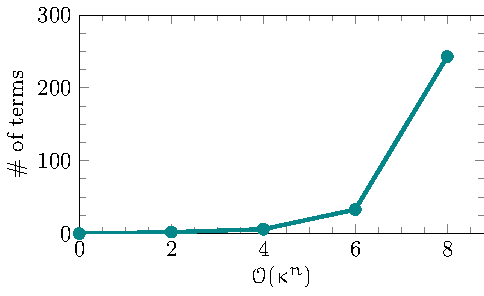
\includegraphics[width=.5\textwidth]{section_3/cluster_number_of_terms}\par}
  \caption{Number of analytic terms from the LCE of the effective theory}
  \label{fig:cluster_num_terms}
\end{figure}

Once more we will compare the effective theory partition function to the one of
the LCE and create a correspondence. We will increase the order of the effective
theory by one, working with $\mathcal{Z}_4$. The method is however easily
generalisable, and the $\mathcal{Z}_8$ effective theory partition function has
been considered for the upcoming result. The $\mathcal{O}(\kappa^4)$ partition
function is
%
\begin{multline}
  \mathcal{Z}_4 = \int [ \mathrm{d} U ]_0 \det{}^{N_f} \qstat \exp \bigg(-\frac{1}{2}
    h_2 N_f \sum_{\langle x,y \rangle} W_{11} (x) W_{11} (y)\\
  + h_2^2 N_f \sum_{\langle x,y \rangle} \sum_{\langle y,z \rangle} W_{11}(x)
    W_{21}(y) W_{11}(z)
  + h_2^2 N_f^2 \sum_{\langle x,y \rangle} W_{21}(x) W_{21}(y) \bigg).
\end{multline}
%
The correspondence is now between the two component field $\phi_i$ in the
following manner
%
\begin{equation}
  \phi_i \Leftrightarrow \big(W_{11}, W_{21}\big)_i\:, \hskip .5cm
  e^{-S_0[\phi]} \Leftrightarrow \mathcal{J} (U_0, W_{11}, W_{21}) \det \qstat
  \:.
\end{equation}
%
The two and three point interactions are given by
%
\begin{equation}
  v_{ij}(x,y) = \delta(\langle x,y \rangle)
    \begin{pmatrix}
      -2 h_2 N_f & 0 \\
      0 & 2 h_2^2 N_f^2
    \end{pmatrix}_{ij}
\end{equation}
%
and
%
\begin{align}
  u_{1jk}(x,y,z) &= 2 h_2^2 N_f 
    \begin{pmatrix}
      0 & \delta(\langle x,z \rangle) \delta(\langle y,z \rangle) \\
      \delta(\langle x,y \rangle) \delta(\langle y,z \rangle) & 0
    \end{pmatrix}_{jk} \;,\\
  u_{2jk}(x,y,z) &= 2 h_2^2 N_f  
  \begin{pmatrix}
    \delta(\langle x,y \rangle) \delta(\langle x,z \rangle) & 0 \\
    0 & \makebox[3cm][c]{$0$}
  \end{pmatrix}_{jk}\;.
\end{align}
%
At $\mathcal{Z}_6$ we see that we have to expand the set of fields to four,
$\phi_i \Leftrightarrow \big(W_{11}, W_{21}, W_{31}, W_{32}\big)_i$,
which would result in the following two point interaction matrix
%
\begin{equation}
  v_{ij}(x,y) = \delta(\langle x,y \rangle)
    \begin{pmatrix}
      -2 h_2 N_f & 0 & 0 & 0\\
      0 & 2 h_2^2 N_f^2 & 0 & 0\\
      0 & 0 & -\textstyle\frac{1}{3} h_2^3 N_f & \textstyle\frac{4}{3} h_2^3 N_f^3\\
      0 & 0 & \textstyle\frac{4}{3} h_2^3 N_f^3 & -\textstyle\frac{1}{3} h_2^3 N_f
    \end{pmatrix}_{ij},
\end{equation}
%
and the other $n$-point functions are too long to list. The computation of the
analytic formula for $\mathcal{W}$ was carried out using all three methods
outlined above (carrying out derivatives, computing graphs directly as well as
using the embedding method). This was done to guarantee correctness of the
result. The number of terms contributing to the analytic function describing
$\mathcal{Z}_{\mathrm{QCD}}$ at a given order in our expansion scheme is plotted
in \figref{fig:cluster_num_terms}, and once more we see that the number of terms
grow exponentially as one increase the order. This necessitates the development
of software to carry out graphical combinatorics to push this to higher orders.
This would e.g. be similar to the work of L\"{u}scher and Weisz in the
groundbreaking work on the $\lambda \phi^4$ lattice theory \citep{Luscher:1988gk,Luscher:1988uq}
where they carried out a LCE to $14$\textsuperscript{th} order to show the
triviality of the theory. One should however note the added difficulty due to
the additional polymer interaction and their geometry. For example the four bond
LCE on a square lattice gives $17$ graphs, while our effective theory has $243$
graphs at the four bond level.

\subsection{Results} \label{sec:cluster_results}

We are now in a position to evaluate thermodynamic functions completely
analytically. Using the LCE we have computed the grand canonical partition
function in the thermodynamic limit though $\kappa^8 u^5$ to first order in
$N_t^{-1}$. We first compare the convergence of the theory in the two parameters
to that obtained through simulating the effective theory. The convergence in the
nearest neighbour effective coupling, $h_2$, is shown in
\figref{fig:analytic_convergeance} (left). Making a comparison to
\figref{fig:numerical_convergence} (left) we see that the analytic convergence
range matches that of the simulated data and shows good quantitative agreement.
In \figref{fig:analytic_convergeance} (right) we see the corresponding
convergence plot in the strong coupling parameter $\beta$. We see that the
analytic computation underestimates the strong coupling contributions. One
should however note the axis scales and note that the finite coupling
corrections are much smaller than the corrections in $\kappa$ and that the main
contribution of finite $\beta$ comes indirectly through a rescaling of the
system.

\begin{figure}
  \begin{center}
    \begin{adjustbox}{max width=\textwidth}
      \includegraphics{section_3/nb_of_h2_beta0}
      \includegraphics{section_3/nb_of_beta}
    \end{adjustbox}
  \end{center}\vskip -.6cm
  \caption{Convergence of the analytic expressions in $h_2$ (left) and $\beta$
    (right) overlayed with the simulation results at highest order. The
    normalised baryon number density has been used in the rightmost plot.}
  \label{fig:analytic_convergeance}
\end{figure}

Next we explore the convergence properties of the theory as we move towards
lighter quarks and smaller lattice sizes. In \figref{fig:convergence_in_spacing}
we plot the baryon number density at lower and lower lattice sizes. The error
bars are estimates of the systematic error given as the difference between two
subsequent orders in the expansion. The first observation is that at
conservative quark masses of $\sim 10 \:\mathrm{GeV}$ we see that the continuum
extrapolation is limited by extrapolation from data taken at $\sim 0.07
\:\mathrm{fm}$. However, we note that in all cases the convergence improves at
higher orders of the expansion, demonstrating the stability of the expansion.
The second observation one can make is that convergence is worse at higher
chemical potential. This combined with the fact that the slope increases makes
accessing the denser systems more difficult. This is a manifestation of fermion
saturation on the lattice, as was discussed in \secref{sec:saturation}.

\begin{figure}[t]
  \begin{center}
    \includegraphics[width=.65\textwidth]{section_3/nb_of_a_mu0999}
  \end{center} \vskip -.5cm
  \caption{Convergence of the baryon number density at smaller and smaller
    lattice spacings. Shows similar limitations to the extrapolation plot of the
  $\mathcal{Z}_2$ theory in \protect\figref{fig:continuum_extrapolation} (left).}\vskip -.2cm
  \label{fig:convergence_in_spacing}
\end{figure}

\begin{figure}
  \begin{center}
    \begin{adjustbox}{max width=\textwidth}
      \includegraphics{section_3/nb_of_mpi_a02}
      \includegraphics{section_3/nb_of_mpi_a01}
    \end{adjustbox}
  \end{center}\vskip -.6cm
  \caption{Order by order convergence as a function of the meson mass of the
    system exposing the heavy quark limits of the system. Left plot at $T = 20\:
    \mathrm{MeV}$ and $a = 0.2\:\mathrm{fm}$, right plot at at $T = 10\:
    \mathrm{MeV}$ and $a = 0.1\:\mathrm{fm}$.}
  \label{fig:convergence_mpi}
\end{figure}

In \figref{fig:convergence_mpi} we plot the convergence of the different orders
of the expansion at varying meson mass at fixed temperature and lattice
spacing. This plot demonstrates the difficulty for the effective theory to reach
smaller quark masses. Although the higher orders does indeed help with the
convergence, we see that the effect of two more orders is small compared to the
relevant scales of the problem. We can therefore not picture an extension to
smaller quark masses through brute force order by order computations.

\subsection{Pad\'e approximants}

An alternative, but very powerful tool for series analyses is the \emph{Pad\'e
approximants}. It is simply a reordering of the power series into a rational
expression
%
\begin{equation}
  [L/M](z) = \frac{a_0 + a_1 z + \dots + a_L z^L}{b_0 + b_1 z + \dots + b_M
    z^M},
\end{equation}
%
so that it's Maclaurin series agrees with the original series to
$(L+M)$\textsuperscript{th} order
%
\begin{equation}
  \sum_{i = 0}^{\mathclap{L+M}} c_i z_i = [L/M](z) + \mathcal{O}(z^{L+M+1}).
\end{equation}
%
An extensive introduction to Pad\'e approximants, their uses and properties
can be found in \citep{Baker:1996cup}. If the approximants are well defined,
they tend to show better convergence properties than their corresponding
Maclaurin series. If one considers a long enough series it is also possible to
use the Pad\'{e} formulation to analyse critical points and non analyticities of
the theory. However one should be careful as the Pad\'{e} series will pick up
both the real physical singularities as well as artefact singularities due to
the fractional nature of the expression. To resolve this one can e.g. study the
different Pad\'e approximants as the $L$-$M$ ratio is a sliding scale. It is
however known that the diagonals ($[L/L]$ and $[L-1/L]$) possess various
favourable properties
\citep[and references therein]{Gaunt:1980zb,Guttmann:1989zb}.

In our case the Pad\'e variable is $h_2$, and the highest order is $L+M = 4$.
After discarding the approximants with artificial singularities we can
compare the convergence to that of the Maclaurin series. This is shown in
\figref{fig:pade_results} (left) where we once more have used the baryon number
density to investigate convergence. We see that the order by order convergence
rate of the Pad\'e approximants are far superior to those of the pure linked
cluster expansion, as is expected. 

\begin{figure}
  \begin{center}
    \begin{adjustbox}{max width=\textwidth}
      \includegraphics{section_3/nb_of_h2_pade}
      \includegraphics{section_3/binding_energy_pade}
    \end{adjustbox}
  \end{center}\vskip -.6cm
  \caption{Results from the Pad\'e approximants. Left: Convergence plot at
    strong coupling compared to the normal series from the LCE. Right: The
    nucleon binding energy as a function of chemical potential at different
    orders.}
  \label{fig:pade_results}
\end{figure}

Finally we plot the binding energy per nucleon, $\epsilon$, as defined
in \meqref{eq:epsilon_definition} with the Pad\'e series in
\figref{fig:pade_results} (right). We observe that this quantity displays the
\emph{silver blaze}, namely that it is zero up until onset transition, where it
in this case becomes negative, as was seen in \citep{Langelage:2014vpa}. With
the fourth order Pad\'e, we can extend the study to higher densities. Although
the quantitative convergence breaks down shortly after the onset transition near
$\mu_B \approx m_B$, we see new qualitative behaviour. In the higher orders we
see that the binding has a minimum and reaches a positive value at growing
chemical potential as is expected from nuclear physics. This means that we have
a qualitative bulk nuclear density, whose qualitative value is still unsettled
by the present study.

We will refrain from analysing any more results until we have introduced a final
improvement to the analytic approach.

\section{Analytic resummation} \label{sec:analytic_resummation}

So far we have managed to analytically calculate the grand canonical potential
of the effective theory to the same order as the effective theory itself, and
consequently achieved access to the thermodynamic quantities analytically.
Although this by itself is both useful due to the permanence of the results, as
well as the additional mathematical insight into the theory it admits, we have
merely reproduced the simulated results. In this section, further improvements to
the theory will be analysed, which will push the analytic evaluation beyond that
of the numerically obtained ones. We will start by introducing a resummation
scheme on the level of the effective theory first in
\secref{sec:chain_resummation}. We will then proceed to a resummation on the
cluster expansion level in \secref{sec:cluster_resummation}. Finally, in
\secref{sec:ladder_resummation}, we will review a second hypothetical
resummation, again on the level of the effective theory.

\subsection{Chain resummation} \label{sec:chain_resummation}

We start with a motivating example. Consider the following four terms from the
effective action \meqref{eq:effective_action_kapp8}
%
\begin{equation}
  h_2 N_f \sum_{\mathrm{dof}} \;
  \begin{tikzpicture}[eft graph, node distance=.4]
    \node[eft node] (n1) {1};
    \node[eft node] (n2) [below=of n1] {1}
      edge[eft bond] (n1);
  \end{tikzpicture}, \;
  - h_2^2 N_f\sum_{\mathrm{dof}}  \:
  \begin{tikzpicture}[eft graph]
    \node[eft node] (n1) {1};
    \node[eft node] (n2) [position=60 degrees from n1] {1}
      edge[eft bond] (n1);
    \node[eft node] (n3) [position=300 degrees from n2] {1}
      edge[eft bond] (n2);
  \end{tikzpicture}, \;
  h_2^3 N_f\sum_{\mathrm{dof}} \:
  \begin{tikzpicture}[eft graph]
    \node[eft node] (n1) {1};
    \node[eft node] (n2) [position=60 degrees from n1] {1}
      edge[eft bond] (n1);
    \node[eft node] (n3) [position=300 degrees from n2] {1}
      edge[eft bond] (n2);
    \node[eft node] (n4) [position=60 degrees from n3] {1}
      edge[eft bond] (n3);
  \end{tikzpicture}, \;
  - h_2^4 N_f\sum_{\mathrm{dof}} \:
  \begin{tikzpicture}[eft graph]
    \node[eft node] (n1) {1};
    \node[eft node] (n2) [position=60 degrees from n1] {1}
      edge[eft bond] (n1);
    \node[eft node] (n3) [position=300 degrees from n2] {1}
    edge[eft bond] (n2);
    \node[eft node] (n4) [position=60 degrees from n3] {1}
      edge[eft bond] (n3);
    \node[eft node] (n5) [position=300 degrees from n4] {1}
      edge[eft bond] (n4);
  \end{tikzpicture} .
\end{equation}
%
It is clear that these four terms follow a common pattern that generates a
chain. Each of the terms above extend the chain by one node while maintaining a
common prefactor. By studying the mathematically equivalent formulation, we
observe that every new link in the chain contributes a factor $h_2 W_{21}$ to
the term, in addition to the necessary spatial geometry. One can check the other
terms in the $\kappa^8$ action, e.g.
%
\begin{equation}
  2 h_2^3 N_f^2 \sum_{\mathrm{dof}} \; \Bigg(
  \begin{tikzpicture}[eft graph]
    \node[eft node] (n1) {1};
    \node[eft node] (n2) [position=60 degrees from n1] {1}
      edge[eft bond, bend left=30]  (n1)
      edge[eft bond, bend right=30] (n1);
    \node[eft node] (n3) [position=300 degrees from n2] {1}
      edge[eft bond] (n2);
  \end{tikzpicture} - 
  \begin{tikzpicture}[eft graph]
    \node[eft node] (n1) {1};
    \node[eft node] (n2) [position=60 degrees from n1] {2}
      edge[eft bond, bend left=30]  (n1)
      edge[eft bond, bend right=30] (n1);
    \node[eft node] (n3) [position=300 degrees from n2] {1}
      edge[eft bond] (n2);
  \end{tikzpicture} \Bigg), \;
  -2 h_2^4 N_f^2 \sum_{\mathrm{dof}} \; \Bigg(
  \begin{tikzpicture}[eft graph]
    \node[eft node] (n1) {1};
    \node[eft node] (n2) [position=60 degrees from n1] {1}
      edge[eft bond, bend left=30]  (n1)
      edge[eft bond, bend right=30] (n1);
    \node[eft node] (n3) [position=300 degrees from n2] {1}
      edge[eft bond] (n2);
    \node[eft node] (n4) [position=60 degrees from n3] {1}
      edge[eft bond] (n3);
  \end{tikzpicture} - 
  \begin{tikzpicture}[eft graph]
    \node[eft node] (n1) {1};
    \node[eft node] (n2) [position=60 degrees from n1] {2}
      edge[eft bond, bend left=30]  (n1)
      edge[eft bond, bend right=30] (n1);
    \node[eft node] (n3) [position=300 degrees from n2] {1}
      edge[eft bond] (n2);
    \node[eft node] (n4) [position=60 degrees from n3] {1}
      edge[eft bond] (n3);
  \end{tikzpicture} \Bigg),
\end{equation}
%
all follow the this pattern. The conjecture is then that every singly connected
node, namely every factor $W_{11}$, can be extended to a chain of arbitrary
length, and that these terms will appear in a predictable form at higher orders.
The chain resummation can schematically be represented as
%
\begin{equation} \label{eq:chain_schematic}
  \tikz[midtikz] \node[inner sep=0pt] (fig) {\includegraphics[scale=1.05]{resummation_schematic}};\;,
\end{equation}
%
in which $\mathcal{C}_0$ represents and arbitrary unsummed term with $m$ singly
connected nodes (\emph{open ends}), and $\mathcal{C}_n$ represents the same term
where the $m$ opens ends have been extended a combined total of $n$ times. We
then sum over the extension $n$ of the $m$ open ends which will result in a
replacement of all open ends
%
\begin{equation} \label{eq:chain_subst}
  W_{11}(x) \to W_{11}(x) \sum_{n=0}^{\infty} \mathcal{G}(\{x_n\}) \prod_{i=1}^{n} (-h_2) W_{21}(x_i).
\end{equation}
%
The factor $\mathcal{G}(\{x_n\})$ represents the geometry of the chain, which we
will later embed onto the polymer linked cluster expansion developed in the
previous section. Before this point we need to review the mathematical structure
of the resummation, and its origin.

\subsubsection{Combinatorial analysis}

We already introduced the combinatorics of the cold and dense regime in
\secref{sec:combinatorics}, which we will build upon in this section. The first
observation we need to make is the types of terms before the spatial gauge link
integrals that contribute to the chain. We will simply state the general pattern
here and prove it later. We define an \emph{open end} to consist of two
consecutive hops that form a pair, such as $1 \, 1$. When we introduced the
pairing notation we used the sixth order single trace as an example, which can
appear in three combinations (as in \meqref{eq:pmpmpm_pairing})
%
\begin{equation}
  \tr \tikz[baseline=-3pt] \matrix [matrix of math nodes,inner sep=1.5pt,ampersand replacement=\&]
    {1 \& 1 \& 2 \& 2 \& 3 \& 3 \\};, \hskip.5cm
  \tr \tikz[baseline=-3pt] \matrix [matrix of math nodes,inner sep=1.5pt,ampersand replacement=\&]
    {1 \& 2 \& 3 \& 3 \& 2 \& 1 \\};, \hskip.5cm
  \tr \tikz[baseline=-3pt] \matrix [matrix of math nodes,inner sep=1.5pt,ampersand replacement=\&]
    {1 \& 2 \& 3 \& 1 \& 2 \& 3 \\};.
\end{equation}
%
The first term has three open ends, the second has two open ends (including cyclic
permutations), while the final term has no open ends. An extension of the chain
is obtained by inserting a new pair in between an already existing open end.
Instead of the quark hopping forth and then directly back again, it will take a
detour through this new position
%
% TODO: Check notation consistency (positions)
\begin{subequations}
  \begin{align}
    \dots
    \tikz[baseline=-3pt]
      \matrix [matrix of math nodes,inner sep=1.5pt,ampersand replacement=\&] {1 \& 1 \\};
    \hspace{.25cm}
    &\tikz
      \draw[->,>=stealth] (0,0) -- +(1cm,0); \hspace{.3cm}
    \dots \: W_{11}(\vec{x}), \\
    \dots
    \tikz[baseline=-3pt]
      \matrix [matrix of math nodes,inner sep=1.5pt,ampersand replacement=\&] {1 \& 2 \& 2 \& 1 \\};
    \hspace{.25cm}
    &\tikz
      \draw[->,>=stealth] (0,0) -- +(1cm,0); \hspace{.3cm}
    \dots \: W_{21}(\vec{x}) W_{11}(\vec{x} + i), \\
    \dots
    \tikz[baseline=-3pt]
      \matrix [matrix of math nodes,inner sep=1.5pt,ampersand replacement=\&] {1 \& 2 \& 3 \& 3\& 2 \& 1 \\};
    \hspace{.25cm}
    &\tikz
      \draw[->,>=stealth] (0,0) -- +(1cm,0); \hspace{.3cm}
    \dots \: W_{21}(\vec{x}) W_{21}(\vec{x} + i) W_{11}(\vec{x} + i + j).
  \end{align}
\end{subequations}
%
The prefactors of terms in this resummation can be calculated from symmetry
arguments.  Assume that we know the symmetry prefactor $1/g$ of a term with $N$
open ends.  Extending one of these can be done in $N/g$ distinct ways, which all
break the previous symmetry. The sum of all such insertions thus have a
prefactor of $N/g$ which is $N$ times that of the base diagram.
However, instead of counting the number of these permutations, one can make the
observation that the problem is equivalent to distributing $n$ indistinguishable
objects to $N$ distinguishable bins. This is assuming that extending any of the
chains give the same result. This is obviously not true in general, as they
result in different geometric objects, however, when we later embed these
objects onto the linked cluster expansion we will only consider the embeddings
in which this discrepancy is irrelevant. In this special case the new symmetry
factor from extending a graph with a symmetry factor $1/g$ with $N$ open ends by
$n$ links is
%
\begin{equation} \label{eq:resummed_symmetry}
  \frac{1}{g'} = \frac{1}{g} \binom{N - 1 + n}{n}\;.
\end{equation}
%
% TODO: Reformulate
This is also only true if we consider a \emph{root graph}, which is any graph
that does not appear as an extension to any other lower order graph. This is
however not a problem as long as we carry out the resummation on an order by
order basis. With this in place we will carry out the gauge integrals
recursively on a chain matrix to show that the above mentioned expression does
indeed appear. As argued, the chain can be expressed as
%
\begin{equation}
  \tikz[baseline=-3pt]
    \matrix [
      matrix of math nodes,
      inner sep=1.5pt,
      ampersand replacement=\&
    ] {X \& 1 \& 2 \& 3 \& 4 \& \dots \& n \& n \& \dots \& 4 \& 3 \& 2 \& 1 \\};,
\end{equation}
%
where $X$ represents the remainder of the term, which may or may not include
additional open ends, and or chains. Since the expression has a recursive
structure it is natural to define the matrices $G_n$ so that
%
\begin{equation}
  \begin{tikzpicture}[baseline={([yshift=-.65ex] nodes.center)}]
    \matrix (nodes) [
      matrix of math nodes,
      inner sep=1.5pt,
      ampersand replacement=\&
    ] {1 \& 2 \& 3 \& 4 \& \dots \& n \& n \& \dots \& 4 \& 3 \& 2 \& 1 \\};
    \draw [
      decorate,
      line width=1.4pt,
      decoration={
        brace,
        mirror,
        amplitude=5pt
      },
    ]
      ([yshift=-.2cm]nodes-1-1.south west) -- ([yshift=-.2cm]nodes-1-12.south east)
      node[midway,below=5pt] {$G_n$};
    \draw [
      decorate,
      line width=1.4pt,
      decoration={
        brace,
        amplitude=5pt
      },
    ]
      ([yshift=.2cm]nodes-1-2.north west) -- ([yshift=.2cm]nodes-1-11.north east)
      node[midway,above=5pt] {$G_{n-1}$};
    \draw [
      decorate,
      line width=1.4pt,
      decoration={
        brace,
        mirror,
        amplitude=5pt
      },
    ]
      ([yshift=-1.1cm]nodes-1-3.south west) -- ([yshift=-1.1cm]nodes-1-10.south east)
      node[midway,below=5pt] {$G_{n-2}$};
  \end{tikzpicture}\; .
\end{equation}
%
The matrix $G_n$ is then defined in terms of $G_{n-1}$. In
\secref{sec:combinatorics} we saw that the static propagator in the cold dense
limit had the approximate expression \meqref{eq:leading_order_static_prop},
meaning that the effecitve hopping matrices take the form
%
\begin{alignat}{99}
  P^{ab}_{\alpha\beta}(y,x) &= \kappa \Big(\frac{1+\gamma_0}{2}\Big)_{\alpha\gamma} K^{ac}_{\vec{x}}(t_y,t_x)
    \sum_{i=1}^3  (1+\gamma_i)_{\gamma\beta} U_{\vec{x},i}^{cb} &&\delta_{\vec{y},\vec{x}+i} \\
  M^{ab}_{\alpha\beta}(y,x) &= \kappa \Big(\frac{1+\gamma_0}{2}\Big)_{\alpha\gamma} K^{ac}_{\vec{x}}(t_y,t_x)
    \sum_{i=1}^3  (1-\gamma_i)_{\gamma\beta} U^{\dagger,cb}_{\vec{x},i} &&\delta_{\vec{y},\vec{x}-i}
\end{alignat}
%
where we have shortened the $K^+$ notation for the brevity. Colour indices are
denoted by Roman characters, while the Driac indices are symbolised by Greek
letters. We also saw in \secref{sec:dirac_indices} that the Dirac trace is
somewhat trivial. The colour matrix content that enters the integrals is thus
%
\begin{equation}
  K^{ac}_{\vec{x}}(t_y,t_x) U^{cb}_{\vec{x},i}, \hskip.5cm\text{and}\hskip.5cm
  K^{ac}_{\vec{x}}(t_y,t_x) U^{\dagger{}, cb}_{\vec{x},i}.
\end{equation}
%
We are now ready to evaluate the colour integrals over the matrix $G_n$
%
\begin{align}
  G_{n}^{af}(t_1,t_2;\vec{x}_0) &= 2 \kappa^2 \sum_{i_0,t_3} \int \mathrm{d} U_{\vec{x}_0,i_0}(t_2) \;
    K_{\vec{x}_0}^{ab}(t_1,t_2)U_{\vec{x}_0,i_0}^{bc}(t_2) \nonumber \\
    &\hspace{3cm}\times G_{n-1}^{cd}(t_2,t_3;\vec{x}_0+i_0) K^{de}_{\vec{x}_0+i_0}(t_3,t_2)
    U_{\vec{x}_0,i_0}^{\dagger,ef}(t_2) \nonumber\\
  &= \frac{2 \kappa^2}{N_c} \sum_{i_0,t_3} K_{\vec{x}_0}^{ab}(t_1,t_2) G_{n-1}^{cd}(t_2,t_3;\vec{x}_0+i)
    K^{de}_{\vec{x}_0+i}(t_3,t_2) \delta_{ce}\delta_{bf} \nonumber\\
  &= \frac{2 \kappa^2}{N_c} \sum_{i_0,t_3} K_{\vec{x}_0}^{af}(t_1,t_2) \tr_c \big[ G_{n-1}(t_2,t_3;\vec{x}_0+i)
    K_{\vec{x}_0+i}(t_3,t_2) \big] \;.\label{eq:chain_integral}
\end{align}
%
The coordinate $\vec{x}_0$ is the coordinate of the beginning of the chain, and
we see that we have a recursive structure for these spatial positions as we move
on the chain $\vec{x}_{m+1} = \vec{x}_m + i_m$. We use the above equation to
define $G_{n-1}$ in terms of $G_{n-2}$
%
\begin{equation}
  G_{n-1}^{ab}(t_2,t_3;\vec{x}_1) = \frac{2 \kappa^2}{N_c} \sum_{i_1,t_4} K_{\vec{x}_1}^{ab}(t_2,t_3)
    \tr_c \big[ G_{n-2}(t_3,t_4;\vec{x}_2) K_{\vec{x}_2}(t_4,t_3) \big]\;.
\end{equation}
%
We insert the expression for $G_{n-1}$ into the one for $G_n$, and get
%
\begin{multline}
  G_{n}^{af}(t_1,t_2;\vec{x}_0)
    = \bigg(\frac{2 \kappa^2}{N_c}\bigg)^2
      \sum_{t_3,t_4} \sum_{i_0,i_1} K_{\vec{x}_0}^{af}(t_1,t_2)
      \tr_c \big[ G_{n-2}(t_3,t_4;\vec{x}_2) K_{\vec{x}_2}(t_4,t_3) \big] \\
  \times
  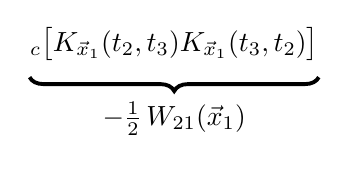
\begin{tikzpicture}[baseline={([yshift=-.5ex] trace.center)}]
    \node[inner sep=0pt] (trace) {%
      $\tr_c \big[ K_{\vec{x}_1}(t_2,t_3) K_{\vec{x}_1}(t_3,t_2)\big]$};
    \draw [
      decorate,
      line width=1.4pt,
      decoration={
        brace,
        mirror,
        amplitude=5pt
      },
    ]
      ([yshift=-.2cm]trace.south west) -- ([yshift=-.2cm]trace.south east)
      node[midway,below=5pt] {$-\frac{1}{2}\,W_{21}(\vec{x}_1)$};
  \end{tikzpicture} \,.
\end{multline}
%
We see that the structure of $G_{n}$ stays the same after one step of the
recursion, except for a factor of $W_{21}$ as well as sums over new degrees of
freedom. The recursion ends at $G_1$, which is the open end of the chain, and is
given by a consecutive, paired hop
%
\begin{align}
  G_{1}^{ae}(\tau_1,\tau_2;\vec{x}_n) &=
    2 \kappa^2 \sum_{i_n} \int \mathrm{d} \vec{U}_{\vec{x}_n,i_n} \, K^{ab}_{\vec{x}_n}(t_1,t_2)
    U_{\vec{x}_n,i_n}^{bc}(t_2) K^{cd}_{\vec{x}_{n+1}}(t_2,t_2)
    U_{\vec{x}_n,i_n}^{\dagger,de}(t_2) \nonumber \\
  &= \frac{2 \kappa^2}{N_c} \sum_{i_n}K^{ae}_{\vec{x}_n}(t_1,t_2)
  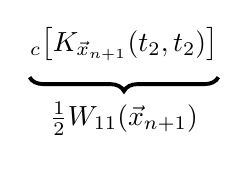
\begin{tikzpicture}[baseline={([yshift=-.5ex] trace.center)}]
    \node[inner sep=0pt] (trace) {%
      $\tr_c \big[ K_{\vec{x}_{n+1}}(t_2,t_2) \big]$};
    \draw [
      decorate,
      line width=1.4pt,
      decoration={
        brace,
        mirror,
        amplitude=5pt
      },
    ]
      ([yshift=-.2cm]trace.south west) -- ([yshift=-.2cm]trace.south east)
      node[midway,below=5pt] {$\frac{1}{2} W_{11}(\vec{x}_{n+1})$};
  \end{tikzpicture} \,. \label{eq:g1_integrated}
\end{align}
%
Recursively inserting the expressions for the $G_{m}$ matrices we obtain a final
result for the full chain matrix
%
\begin{multline}
  G_{n}^{ab}(t_1,t_2;\vec{x}_0) =
    K_{\vec{x}_0}^{ab}(t_1,t_2) \bigg(\frac{2 \kappa^2}{N_c}\bigg)^n
    \sum_{\substack{t_3,t_4,\\\dots,t_{n+1}}}
    \sum_{\substack{i_0,i_1,\\\dots,i_n}}
      W_{11}(\vec{x}_{n+1}) \prod_{k=2}^{n} \big(-W_{21}(\vec{x}_k)\big) \\
  =K_{\vec{x}_0}^{ab}(t_1,t_2) \bigg(\frac{2 \kappa^2}{N_c}\bigg)^n 
  N_{t}^{n-1} \sum_{\substack{i_0,i_1,\\\dots,i_n}}
    W_{11}(\vec{x}_{n+1}) \prod_{k=2}^{n} \big(-W_{21}(\vec{x}_k)\big)\;. \label{eq:full_gn}
\end{multline}
%
The sums over the temporal variables could be trivially evaluated as the
$W_{nm}$ factors are independent of their time argument.

To tie it all together let us consider a generic contribution which has $N$ open
ends
%
\begin{equation} \label{eq:chain_begin}
  \mathcal{C}_0 = \frac{1}{g} \tr \big[
    G_1(t_1,t_2;\vec{x}_1) M_1 G_1 (t_3,t_4;\vec{x}_2) M_2 \cdots
    G_1 (t_{2N-1},t_{2N};\vec{x}_N) M_N
  \big]\;,
\end{equation}
%
where the matrices $M_i$ are the rest of the term, comparable to the left hand
side of \meqref{eq:chain_schematic}. We have only considered a single trace term
here, however the analysis can be easily extended to multi trace terms as a
chain can only reside within one fermion trace. Inserting the expression for
$G_1$ gives
%
\begin{multline}
  \mathcal{C}_0 =
    \frac{1}{g} \tr \big[
      K(t_1,t_2;\vec{x}_1) M_1 K(t_3,t_4;\vec{x}_2) M_2
      \cdots K(t_{2N-1},t_{2N};\vec{x}_N) M_N
    \big] \\
  \times \bigg(\frac{\kappa^2}{N_c}\bigg)^N\;\sum_{\mathclap{i_1,i_2,\dots,i_N}}
    W_{1,1}(\vec{x}_1 + i_1) W_{1,1}(\vec{x}_2 + i_2) 
    \cdots W_{1,1}(\vec{x}_N + i_N).
\end{multline}
%
We can now attach chains of length $n_i$ to each of the $N$ open ends so that
the total length of the chain is $n$, corresponding to the right hand side of
\meqref{eq:chain_schematic}
%
\begin{multline}
  \mathcal{C}_n =
    \hskip .2cm\sum_{\mathclap{n_1,n_2,\dots,n_N}} \hskip .5cm
      \frac{1}{g_{\{n_i\}}}
      \tr \big[
        G_{n_1 + 1}(t_1,t_2;\vec{x}_1) M_1
        G_{n_2+1} (t_3,t_4;\vec{x}_2) M_2 \\ 
        \cdots \times G_{n_N + 1} (t_{2N-1},t_{2N};\vec{x}_N) M_N
      \big]
    \delta\Big(\scalemath{0.8}{\sum_{i=1}^N n_i - n}\Big).
\end{multline}
%
This gives a symmetry factor that depends on the partitioning of the attachments
$\{n_i\}$.  We insert the expression for $G_n$ from \meqref{eq:full_gn}, which
gives us
%
\begin{multline}
  \mathcal{C}_n =
    \hskip .2cm\sum_{\mathclap{n_1,n_2,\dots,n_N}} \hskip .5cm
      \frac{1}{g_{\{n_i\}}}
      \tr \big[
        K(t_1,t_2;\vec{x}_1) M_1 K(t_3,t_4;\vec{x}_2) M_2 \cdots
        K(t_{2N-1},t_{2N};\vec{x}_N) M_N
      \big]\\
  \times \bigg(\frac{\kappa^2}{N_c}\bigg)^{N+\mathrlap{n}}
    N_{t}^n \sum_{\{\vec{x}_i\}} \prod_{j=1}^N W_{1,1}(\vec{x}_{j (n_j+1)})
    \prod_{k=0}^{n_j} \big(-W_{2,1}(\vec{x}_{j k})\big) \;
    \delta\Big(\scalemath{0.8}{\sum_{i=1}^N n_i - n}\Big),
\end{multline}
%
where we once more have introduced recursive coordinate vectors
$\vec{x}_{i(j+1)} = \vec{x}_{ij} + i_{ij}$ which originate from the base
position $\vec{x}_{i0} \equiv \vec{x}_i$. There is a remaining sum over all
geometries of the extended graphs through the variables $\{\vec{x}_i\}$ which we
have to examine further.  We see that the base diagram, what is explicitly left
in the trace, is the same for the term with and without attachments, which is
the crucial observation necessary for the correctness of the chain resummation.

\subsubsection{Embeddings}

To be able to say anything about the final sum over the chain positions we once
more turn to the graph- and lattice embeddings. The snaking chain is in no way a
foreign principle to the LCE, as it is the basic ingredient for cluster
expansion resummation schemes, which we will analyse further in the next
section. For now it is enough to know that for every chain graph there exists a
skeleton graph with the appropriate geometry. For example,
%
\begin{equation} \label{eq:skeleton_chains}
  \tikz[midtikz] \node[inner sep=0pt] (fig) {%
    \includegraphics[scale=1.05]{valid_skeleton_chains}};\;,
\end{equation}
%
all have the proper geometry to have a chain embedded onto them, assuming that
\tikz \node[outer 2, fill=ColourHl1] {}; denotes a suitable \emph{graph
  remainder}. The sum over all valid skeleton graphs is unfortunately an
impossible task, and we will have to restrict the analysis to a subset of the
graphs we can compute. One such set is all graphs where the chain never overlaps
with itself, nor the graph remainder. We can thus apply this resummation scheme
to all embeddings and combinations of graphs entering into the full
$\mathcal{O}(\kappa^8)$ polymeric linked cluster expansion. This includes direct
map embeddings such as
%
\begin{equation}
  \begin{tikzpicture}[graph style,node distance=.4]
  \node[inner 1] (n1) {};
  \node[inner 1] (n2) [position=330 degrees from n1] {}
    edge[bond 1] (n1);
  \node[inner 1] (n3) [position=90 degrees from n1] {}
    edge[bond 1] (n1);
  \node[inner 1] (n4) [position=210 degrees from n1] {}
    edge[bond 1] (n1);
\end{tikzpicture}
\:+\: 3\:
\begin{tikzpicture}[graph style,node distance=.4]
  \node[inner 1] (n1) {};
  \node[inner 1] (n2) [position=330 degrees from n1] {}
    edge[bond 1] (n1);
  \node[inner 1] (n5) [position=60 degrees from n2] {}
    edge[bond 1] (n2);
  \node[inner 1] (n3) [position=90 degrees from n1] {}
    edge[bond 1] (n1);
  \node[inner 1] (n4) [position=210 degrees from n1] {}
    edge[bond 1] (n1);
\end{tikzpicture}
\:+\: 3\:
\begin{tikzpicture}[graph style,node distance=.4]
  \node[inner 1] (n1) {};
  \node[inner 1] (n2) [position=330 degrees from n1] {}
    edge[bond 1] (n1);
  \node[inner 1] (n5) [position=60 degrees from n2] {}
    edge[bond 1] (n2);
  \node[inner 1] (n3) [position=90 degrees from n1] {}
    edge[bond 1] (n1);
  \node[inner 1] (n6) [position=180 degrees from n3] {}
    edge[bond 1] (n3);
  \node[inner 1] (n4) [position=210 degrees from n1] {}
    edge[bond 1] (n1);
\end{tikzpicture}
\:+\: 3\:
\begin{tikzpicture}[graph style,node distance=.4]
  \node[inner 1] (n1) {};
  \node[inner 1] (n2) [position=330 degrees from n1] {}
    edge[bond 1] (n1);
  \node[inner 1] (n5) [position=60 degrees from n2] {}
    edge[bond 1] (n2);
  \node[inner 1] (n6) [position=300 degrees from n5] {}
    edge[bond 1] (n5);
  \node[inner 1] (n3) [position=90 degrees from n1] {}
    edge[bond 1] (n1);
  \node[inner 1] (n4) [position=210 degrees from n1] {}
    edge[bond 1] (n1);
\end{tikzpicture}
\hskip 1ex\tikz[baseline=-.25em] \draw[-{Stealth[round]},line width=.7pt] (0,0) -- (1,0); \hskip 1ex
\begin{tikzpicture}[graph style,node distance=.4]
  \node[inner 1] (n1) {};
  \node[resum node] (n2) [position=330 degrees from n1] {}
    edge[bond 1] (n1);
  \node[resum node] (n3) [position=90 degrees from n1] {}
    edge[bond 1] (n1);
  \node[resum node] (n4) [position=210 degrees from n1] {}
    edge[bond 1] (n1);
\end{tikzpicture}
\;, 
\end{equation}
%
embeddings where the overlap only appears in sections of the diagram to highest
order,
%
\begin{equation}
  \begin{tikzpicture}[graph style]
  \node[inner 1] (n1) {};
  \node[outer 1] (n1o) at (n1) {};
  \node[inner 1] (n2) [position=60 degrees from n1] {}
    edge[bond 1, bend left=45]  (n1o)
    edge[bond 1, bend right=45] (n1o);
  \node[inner 1] (n3) [position=300 degrees from n2] {}
    edge[bond 1] (n2);
\end{tikzpicture}
\:+\:
\begin{tikzpicture}[graph style]
  \node[inner 1] (n1) {};
  \node[outer 1] (n1o) at (n1) {};
  \node[inner 1] (n2) [position=60 degrees from n1] {}
    edge[bond 1, bend left=45]  (n1o)
    edge[bond 1, bend right=45] (n1o);
  \node[inner 1] (n3) [position=300 degrees from n2] {}
    edge[bond 1] (n2);
  \node[inner 1] (n4) [position=60 degrees from n3] {}
    edge[bond 1] (n3);
\end{tikzpicture}
\:+\:
\begin{tikzpicture}[graph style]
  \node[inner 1] (n1) {};
  \node[outer 1] (n1o) at (n1) {};
  \node[inner 1] (n2) [position=60 degrees from n1] {}
    edge[bond 1, bend left=45]  (n1o)
    edge[bond 1, bend right=45] (n1o);
  \node[inner 1] (n3) [position=300 degrees from n2] {}
    edge[bond 1] (n2);
  \node[inner 1] (n4) [position=60 degrees from n3] {}
    edge[bond 1] (n3);
  \node[inner 1] (n5) [position=300 degrees from n4] {}
    edge[bond 1] (n4);
\end{tikzpicture}
\hskip 1ex\tikz[baseline=-.25em] \draw[-{Stealth[round]},line width=.7pt] (0,0) -- (1,0); \hskip 1ex
\begin{tikzpicture}[graph style]
  \node[inner 1] (n1) {};
  \node[outer 1] (n1o) at (n1) {};
  \node[inner 1] (n2) [position=60 degrees from n1] {}
    edge[bond 1, bend left=45]  (n1o)
    edge[bond 1, bend right=45] (n1o);
  \node[resum node] (n3) [position=300 degrees from n2] {}
    edge[bond 1] (n2);
\end{tikzpicture}
\;, 
\end{equation}
%
and finally multi-diagram embeddings with free ends
%
\begin{equation}
  \begin{tikzpicture}[graph style]
  \node[inner 1] (n1) {};
  \node[inner 1] (n2) [position=60 degrees from n1] {};
  \node[outer 2] (n2o) at (n2) {}
    edge[bond 1] (n1);
  \node[inner 2] (n3) [position=300 degrees from n2] {};
  \node[outer 1] (n3o) at (n3) {}
    edge[bond 1, bend left=45]  (n2o)
    edge[bond 2, bend right=45] (n2o);
  \node[inner 2] (n4) [position=60 degrees from n3] {}
    edge[bond 2] (n3o);
\end{tikzpicture}
\:+\: 2\:
\begin{tikzpicture}[graph style]
  \node[inner 1] (n1) {};
  \node[inner 1] (n2) [position=60 degrees from n1] {};
  \node[outer 2] (n2o) at (n2) {}
    edge[bond 1] (n1);
  \node[inner 2] (n3) [position=300 degrees from n2] {};
  \node[outer 1] (n3o) at (n3) {}
    edge[bond 1, bend left=45]  (n2o)
    edge[bond 2, bend right=45] (n2o);
  \node[inner 2] (n4) [position=60 degrees from n3] {}
    edge[bond 2] (n3o);
  \node[inner 2] (n5) [position=300 degrees from n4] {}
    edge[bond 2] (n4);
\end{tikzpicture}
\:+\:
\begin{tikzpicture}[graph style]
  \node[inner 1] (n1) {};
  \node[inner 1] (n2) [position=60 degrees from n1] {};
  \node[outer 2] (n2o) at (n2) {}
    edge[bond 1] (n1);
  \node[inner 2] (n3) [position=300 degrees from n2] {};
  \node[outer 1] (n3o) at (n3) {}
    edge[bond 1, bend left=45]  (n2o)
    edge[bond 2, bend right=45] (n2o);
  \node[inner 2] (n4) [position=60 degrees from n3] {}
    edge[bond 2] (n3o);
  \node[inner 2] (n5) [position=300 degrees from n4] {}
    edge[bond 2] (n4);
  \node[inner 1] (n6) [position=120 degrees from n1] {}
    edge[bond 1] (n1);
\end{tikzpicture}
\:+\: 2\:
\begin{tikzpicture}[graph style]
  \node[inner 1] (n1) {};
  \node[inner 1] (n2) [position=60 degrees from n1] {};
  \node[outer 2] (n2o) at (n2) {}
    edge[bond 1] (n1);
  \node[inner 2] (n3) [position=300 degrees from n2] {};
  \node[outer 1] (n3o) at (n3) {}
    edge[bond 1, bend left=45]  (n2o)
    edge[bond 2, bend right=45] (n2o);
  \node[inner 2] (n4) [position=60 degrees from n3] {}
    edge[bond 2] (n3o);
  \node[inner 2] (n5) [position=300 degrees from n4] {}
    edge[bond 2] (n4);
  \node[inner 2] (n6) [position=60 degrees from n5] {}
    edge[bond 2] (n5);
\end{tikzpicture}
\hskip 1ex\tikz[baseline=-.25em] \draw[-{Stealth[round]},line width=.7pt] (0,0) -- (1,0); \hskip 1ex
\begin{tikzpicture}[graph style]
  \node[resum node] (n1) {};
  \node[inner 1] (n2) [position=60 degrees from n1] {};
  \node[outer 2] (n2o) at (n2) {}
    edge[bond 1] (n1);
  \node[inner 2] (n3) [position=300 degrees from n2] {};
  \node[outer 1] (n3o) at (n3) {}
    edge[bond 1, bend left=45]  (n2o)
    edge[bond 2, bend right=45] (n2o);
  \node[resum node] (n4) [position=60 degrees from n3] {}
    edge[bond 2] (n3o);
\end{tikzpicture}
\;.
\end{equation}
%
We have introduced the symbol
\,\tikz \node[resum node,scale=1.6] {};\, to indicate a resummed open end in our
diagrammatic representation. For this subset of all possible embeddings of the
chain, the integrals, embedding factors and symmetry factors can be computed.

We finish the computation of the resummed graph $\mathcal{C}_n$ with this
restricted set of embeddings, and label this set $\mathcal{C}_n^*$. The total
symmetry factor after summing over the extension partitions $\{n_i\}$ are
exactly the ones we argued for in \meqref{eq:resummed_symmetry}
%
\begin{equation}
  \sum_{\mathclap{n_1,n_2,\dots,n_N}}  \hskip .5cm \frac{1}{g_{\{n_i\}}} = \frac{1}{g} \binom{N-1+n}{n}\;.
\end{equation}
%
The spatial integral over the $\mathcal{C}_n^*$ is
%
\begin{multline}
  \int [\mathrm{d} U]_0 \, \mathcal{C}_n^*
  = \frac{1}{g} \binom{N-1+n}{n} \Omega \int [\mathrm{d} U]_0 \, \det{}^{N_f}\big[Q_{\mathrm{stat}}\big]
    \tr \big[ K_1 M_1 K_2 M_2 \cdots K_N M_N  \big] \\
  \times \bigg(\frac{2d \kappa^2}{N_c}\int [\mathrm{d} U]_0 \,
    \det{}^{N_f}\big[Q_{\mathrm{stat}}\big] W_{11}\bigg)^N
  \bigg(\minus{}\frac{2d \kappa^2N_{\tau}}{N_c}\int [\mathrm{d} U]_0 \,
      \det{}^{N_f}\big[Q_{\mathrm{stat}}\big] W_{21}\bigg)^{\mathrlap{n}}\;.
\end{multline}
%
Here $\Omega$ is the embedding factor of the base diagram, and every new node in
the chain will contribute with a lattice embedding of $(2d)$ as discussed in
\secref{sec:classical_lce_nn}. The integrals over $W_{11}$ and $W_{21}$ is
nothing but the previously defined $z$-functions. Finally we sum over the total
length of the attachments $n$
%
\begin{multline}
  \sum_{n=0}^{\infty} \int [\mathrm{d} U]_0 \mathcal{C}_n^*
    = \frac{1}{g} \int [\mathrm{d} U]_0 \bar{\mathcal{C}}_0^*\:
    \Big(\frac{(2d) \kappa^2}{N_c} z_{(11)}\Big)^N
    \sum_{n=0}^{\infty} \binom{N-1+n}{n} \big(-(2d) h_2\, z_{(21)}\big)^n \\
  = \frac{1}{g} \int [\mathrm{d} U]_0 \bar{\mathcal{C}}_0^*\:
  \bigg(\frac{(2d) \kappa^2}{N_c} \frac{z_{(11)}}{1 + (2d) h_2\, z_{(21)}} \bigg)^{\mathrlap{N}}.
\end{multline}
%
To highlight the substitution we have extracted the open ends from the base
graph $\mathcal{C}_0$, and named the remainder $\bar{\mathcal{C}}_0$. This final
equation proves the resummation identity in \meqref{eq:chain_subst}. At the
linked cluster level we make the substitution
%
\begin{equation}
  z_{(11)} \hskip .1cm\to\hskip .1cm \frac{z_{(11)}}{1 + (2d) h_2\, z_{(21)}},
\end{equation}
%
at an order by order level, making sure we remove the appropriate higher order
graphs this resummation predicts. A demonstration of the convergence power of
resummation is shown in \figref{fig:resummation_demonstration} (left), where we
have plotted the contribution to the baryon number density of the single chain,
single graph terms. We plot the full result up the highest known order as well
as higher order truncated results from the resummation formula, and the resummed
result itself. We see that the different orders diverge to $\pm \infty$ at some
point at increasing values of $h_2$ while the full resummed result stays under
control.

\begin{figure}
  \begin{center}
    \begin{adjustbox}{max width=\textwidth}
      \includegraphics{section_4/resummed_nb_test_single_chain}
      \includegraphics{section_4/M_cumulants}
    \end{adjustbox}
  \end{center}\vskip -.6cm
  \caption{Left: Known and predicted contributions to baryon number density for
  a single chain single graph embedding. Right: The $M$-cumulants as a function
  of $h_1$ for three different embedding types.}
  \label{fig:resummation_demonstration}
\end{figure}

Finally, the systematic errors introduced by the resummation need to be
discussed. In the resummation scheme we chose a specific embedding for the
higher order graphs while neglecting other embeddings at the same order. Due to
the nature of the method of moments and cumulants this results in a slight
overcounting of the number of terms as the embedding factor $(2d)^n$ will
naturally include geometries that overlap with itself. One possible way to
rectify this is to change the embedding factor to the correct one, given by the
theory of the \emph{Self-Avoiding Walk} see e.g. \citep{Rensburg:2009jpa} for a
review. This is however not the preferred aproach as it would spoil the nice
properties of the cluster expansion. We rather regard the cumulants as the
primitive objects of the theory, for which the embedding factor is correct. One
might then study the amplitude of the corrections appearing at the same orders
as the chain elements. In \figref{fig:resummation_demonstration} (right) we plot
the value of three cumulants as a function of of their primary variable, $h_1$.
We see that the free value is for all values of $h_1$ at least one order of
magnitude higher than its overlapping counterparts. This behaviour is due to the
fact that the integrals
%
\begin{equation}
  \int \mathrm{d} L \, W_{nm}^N, \hskip .5cm\text{and}\hskip .5cm
  \bigg(\int \mathrm{d} L \, W_{nm} \bigg)^N,
\end{equation}
%
are of the same order of magnitude, resulting in cancellations in the cumulants.
This gives us additional confidence in the resummation, and shows that the
systematic errors are small.

\subsection{Cluster resummation} \label{sec:cluster_resummation}

As mentioned earlier, the idea of graph level resummation schemes has been
around for the LCE since its conception \citep[see e.g.][for a review]{Wortis:1980zb}, and
the same machinery is to some extent applicable here as well. We will
nonetheless choose a simpler approach to LCE resummations that complements the
already incorporated chain resummation. In the previous section we analysed how
to create chains on the level of the effective theory. This is however not the
only way of creating chains. Instead of extending the base diagrams at the
pre-integral level, one can create chains with the LCE ingredients themselves. For
example a chain of lowest order nearest neighbour interactions
%
\begin{equation}
  \begin{tikzpicture}[graph style]
    \node[outer 2,fill=ColourHl1] (n1) {};
    \node[outer 1] (n2) [position=60 degrees from n1] {}
      edge[bond 1] (n1);
    \node[inner 1] at (n2) {};
    \node[outer 1] (n3) [position=300 degrees from n2] {}
      edge[bond 1] (n2);
    \node[inner 1] at (n3) {};
    \node[inner sep=2pt,circle,draw,thin,densely dotted] (n4) [position=60 degrees from n3] [scale=0.5] {$\cdots$}
      edge[bond 1] (n3);
    \node[outer 1] (n5) [position=300 degrees from n4] {}
      edge[bond 1] (n4);
    \node[inner 1] at (n5) {};
    \node[outer 1] (n6) [position=60 degrees from n5] {}
      edge[bond 1] (n5);
    \node[inner 1] at (n6) {};
    \node[outer 1] (n7) [position=300 degrees from n6] {}
      edge[bond 1] (n6);
    \node[inner 1] at (n7) {};
    \node[inner sep=2pt,circle,draw,thin,densely dotted] (n8) [position=60 degrees from n7] [scale=0.5] {$\cdots$}
      edge[bond 1] (n7);
    \node[outer 1] (n9) [position=300 degrees from n8] {}
      edge[bond 1] (n8);
    \node[inner 1] at (n9) {};
    \node[outer 1] (n10) [position=60 degrees from n9] {}
      edge[bond 1] (n9);
    \node[inner 1] at (n10) {};
    \node[outer 1] (n11) [position=300 degrees from n10] {}
      edge[bond 1] (n10);
    \node[inner 1] at (n11) {};
  \end{tikzpicture}
\end{equation}
%
Further improvements is gained by mixing the two expansion schemes and extending
every open end by all combinations of chain segments resulting in a chain of a
certain length
%
\begin{equation}
  \begin{tikzpicture}[graph style, baseline={([yshift=.5ex] n1.center)}]
    \node[outer 2,fill=ColourHl1] (n1) {};
    \node[inner 1] (n2) [position=60 degrees from n1] {}
      edge[bond 1] (n1);
    \node[inner 1] (n3) [position=300 degrees from n2] {}
      edge[bond 1] (n2);
    \node[inner sep=2pt,circle,draw,thin,densely dotted] (n4) [position=60 degrees from n3] [scale=0.5] {$\cdots$}
      edge[bond 1] (n3);
    \node[outer 2] (n5) [position=300 degrees from n4] {}
      edge[bond 1] (n4);
    \node[inner 1] at (n5) {};
    \node[inner 2] (n6) [position=60 degrees from n5] {}
      edge[bond 2] (n5);
    \node[inner 2] (n7) [position=300 degrees from n6] {}
      edge[bond 2] (n6);
    \node[inner sep=2pt,circle,draw,thin,densely dotted] (n8) [position=60 degrees from n7] [scale=0.5] {$\cdots$}
      edge[bond 2] (n7);
    \node[inner 3] (n9) [position=300 degrees from n8] {}
      edge[bond 3] (n8);
    \node[inner 3] (n10) [position=60 degrees from n9] {}
      edge[bond 3] (n9);
    \node[inner 3] (n11) [position=300 degrees from n10] {}
      edge[bond 3] (n10);

    \draw [
      decorate,
      line width=1.0pt,
      decoration={
        brace,
        mirror,
        amplitude=5pt
      },
    ]
      ([yshift=-.2cm] n1.center) -- ([yshift=-.2cm] n5.center)
      node[midway,below=7.5pt,scale=0.65] {chain $1$};

    \draw [
      decorate,
      line width=1.0pt,
      decoration={
        brace,
        amplitude=5pt
      },
    ]
      ([yshift=.3cm] n4.center -| n5.center) -- ([yshift=.3cm] n8.center)
      node[midway,above=7.5pt,scale=0.65] {chain $2$};

    \draw [
      decorate,
      line width=1.0pt,
      decoration={
        brace,
        mirror,
        amplitude=5pt
      },
    ]
      ([yshift=-.2cm] n9.center -| n8.center) -- ([shift={(2pt,-.2cm)}] n11.center)
      node[midway,below=7.5pt,scale=0.65] {chain $m$};

  \end{tikzpicture}
\end{equation}
%
This can most easily be achieved by partitioning a chain into $m \in [1,n]$
smaller chains . E.g. one such partition with $m = 4$, $n = 6$, is
%
\begin{equation}
  \begin{tikzpicture}[graph style,node distance=0.5,baseline={([yshift=-.5ex]n0.center)}]
    \node[outer 2, fill=ColourHl1] (n0) {};
    \foreach \x in {1,...,6} {%
      \pgfmathparse{\x-1}
      \edef\y{\pgfmathresult}
      \node[inner 1] (n\x) [right=of n\y] {}
        edge[bond 1] (n\y);
    }
    \draw[{Stealth[round]}-,thick] ([yshift=-.2cm] n2.center) -- +(0,-.4cm);
    \draw[{Stealth[round]}-,thick] ([yshift=-.2cm] n3.center) -- +(0,-.4cm);
    \draw[{Stealth[round]}-,thick] ([yshift=-.2cm] n5.center) -- +(0,-.4cm);
  \end{tikzpicture}
  \hskip .5cm\to\hskip .5cm
  \begin{tikzpicture}[graph style,node distance=0.5,baseline={([yshift=-.5ex]n0.center)}]
    \node[outer 2, fill=ColourHl1] (n0) {};
    \node[inner 1] (n1) [right=of n0] {}
      edge[bond 1] (n0);
    \node[inner 1] (n2i) [right=of n1] {};
    \node[outer 2] (n2) at (n2i) {}
      edge[bond 1] (n1);
    \node[inner 2] (n3i) [right=of n2] {};
    \node[outer 3] (n3) at (n3i) {}
      edge[bond 2] (n2);
    \node[inner 3] (n4) [right=of n3] {}
      edge[bond 3] (n3);
    \node[inner 3] (n5i) [right=of n4] {};
    \node[outer 4] (n5) at (n5i) {}
      edge[bond 3] (n4);
    \node[inner 4] (n6) [right=of n5] {}
      edge[bond 4] (n5);
  \end{tikzpicture} \;.
\end{equation}
%
Every cut in the chain will replace a $-h_2 W_{21}$ in the chain formula by a
factor $-2 h_2 N_f W_{(11)^2}$, and $m$ replacements on a $n$ long chain can be
done in $\binom{n}{m}$ ways. The combined cluster and chain resummation formula
is therefore summarised as the replacement
%
\begin{multline}
  z_{(11)} \hskip .2cm\to\hskip .2cm z_{(11)} \sum_{n=0}^{\infty} 
    \sum_{m=0}^{n} \binom{n}{m} (-(2d)h_2)^{n+m}\, z_{(21)}^n\, (N_f z_{(11)^2})^m \\
  = \frac{z_{(11)}}{1 + 2 N_f (2d) h_2\, z_{(11)^2} + (2d) h_2\, z_{(21)}}.
\end{multline}
%
As this is only a fraction of the full LCE resummation scheme, further
improvements are expected to appear as one eventually crancks the machinery.
However this particular subset of cluster resummations synergise well with the
already developed chain resummation.

\subsection{Ladder resummation} \label{sec:ladder_resummation}

The last of the resummation schemes addressed in this thesis is a \emph{ladder
resummation}, which simply is a renormalisation scheme for the nearest neighbour
coupling constant. The idea behind the ladder resummation is, similar to the
chain resummation, simple, albeit mathematically complicated. The general
principle is sketched in \figref{fig:ladder_schematic}, in
which all the details are suppressed. The full ladder is given by the nearest
neighbour kinetic determinant
%
\begin{equation}
  \prod_i \det (1 - \kappa^2 P_i M_i) \equiv \det (1 - \kappa^2 \mathcal{M}_{C_2}),
\end{equation}
%
which represents a different ordering scheme of the spatial hopping expansion.
It is possible to express the full static determinant in this path ordering
scheme, which is equivalent to the hopping scheme we have used so far. We adopt
the same notation as in \citep{Rindlisbacher:2015pea}
%
\begin{equation}
  \det \qkin = \prod_{n} \prod_{\{C_n\}} \det(1 - \kappa^n \mathcal{M}_{C_n}),
\end{equation}
%
in which $C_s$ symbolises a spatial path of length $s$ and the product goes over
all such paths. The path ordered determinants can then be expanded in traces
using the \emph{Faddeev-LeVerrier algorithm}, which truncates at the dimension
of the matrix. This formalism does however in no way simplify the computation of
the effective theory as the combinatorics of the spatial gauge integrals, which
presents the higher obstacle, remain.

\begin{figure}[t]
  \begin{center}
    \includegraphics[scale=1.5]{ladder_resummation_schematic}
  \end{center}
  \caption{The ladder resummation graphic, illustrating the general principle.}
  \label{fig:ladder_schematic}
\end{figure}

Expanding the nearest neighbour path determinant gives
%
\begin{multline}
  \det(1 - \kappa^2 \mathcal{M}_{C_2}) = 1 - \kappa^2 \tr(\mathcal{M}_{C_2})
  -\frac{1}{2} \kappa^4 \big( \tr(\mathcal{M}_{C_2}^2) - \big(\tr(\mathcal{M}_{C_2})\big)^2 \big) \\
  -\frac{1}{6} \kappa^6 \big( \big(\tr(\mathcal{M}_{C_2})\big)^3 - 3 \tr
  (\mathcal{M}_{C_2}) \tr (\mathcal{M}_{C_2}^2) + 2 \tr (\mathcal{M}_{C_2}^3)
  \big) + \dots
\end{multline}
%
which grants some insight into the terms that will appear in the ladder. It is
however impossible to compute the full ladder, and we will have to settle for a
computable subset of all graphs. One possible subset is the single trace terms
%
\begin{equation}
  \sum_i \tr ( P_i M_i P_i M_i P_i M_i \cdots )
\end{equation}
%
which will include both high order coupled terms as well as close packed
embeddings of longer chains. For example the chains of the previous expansion
will be one such term, where the chain has been folded onto a nearest neighbour
pair. On top of being restricted by combinatorics, we are also restricted by
integrability of the linked cluster integrals. The chain had the advantage that
no new integrals ($z$-functions) are needed, while in a nearest neighbour
resummation, new integrals will inevitably appear. We therefore turn to an even
smaller subset of all nearest neighbour graphs, namely
%
\begin{equation}
  \tr( \tikz[baseline=-3pt] \matrix [matrix of math nodes,inner sep=1.5pt,ampersand replacement=\&]
    {1 \& 1 \& 2 \& 2 \& 3 \& 3 \& 4 \& 4 \& 5 \& 5 \& \dots \& n \& n\\};).
\end{equation}
%
By earlier analysis we know that these diagrams have $n$ open ends and thus
represent the set of \emph{star graphs}
%
\begin{equation}
  \begin{tikzpicture}[graph style,node distance=.4]
    \node[regular polygon, regular polygon sides=4, minimum size=1cm] (gon1) at (0,0) {};
    \node[skeleton node] (n11) at (gon1.north) {};
    \node[skeleton node] (n12) at (gon1.south) {}
      edge[skeleton bond] (n11);

    \node[regular polygon, regular polygon sides=4, minimum size=1cm] (gon2) at (2cm,0) {};
    \node[skeleton node] (n20) at (gon2.center) {};
    \node[skeleton node] (n21) at (gon2.corner 1) {}
      edge[skeleton bond] (n20);
    \node[skeleton node] (n22) at (gon2.corner 3) {}
      edge[skeleton bond] (n20);

    \foreach \s in {3,...,6} {
      \node[regular polygon, regular polygon sides=\s, minimum size=1cm] (gon\s) at ($(-2cm,0) + (2cm*\s,0)$) {};
      \node[skeleton node] (n\s0) at (gon\s.center) {};
      \foreach \i in {1,...,\s} {
        \node[skeleton node] (n\s\i) at (gon\s.corner \i) {}
          edge[skeleton bond] (n\s0);
      }
    }
    \node at (11.25cm, 0) {$\cdots$};
  \end{tikzpicture}
\end{equation}
%
The structure is the same as a consecutive set of $G_1$ matrices from earlier
%
\begin{equation}
  \mathcal{A}_n = 
  \tr( \tikz[baseline=-3pt] \matrix [matrix of math nodes,inner sep=1.5pt,ampersand replacement=\&]
    {1 \& 1 \& 2 \& 2 \& \dots \& n \& n\\};) =
  \begin{tikzpicture}[baseline={([yshift=-.5ex] trace.center)}]
    \node[inner sep=0pt] (trace) {%
      $\tr( G_1 G_1 \cdots G_1)$};
    \draw [
      decorate,
      line width=1.4pt,
      decoration={
        brace,
        mirror,
        amplitude=5pt
      },
      transform canvas={yshift=-.2cm},
    ]
      (trace.south west) -- (trace.south east)
      node[midway,below=5pt] {$n$ times};
  \end{tikzpicture} \,
\end{equation}
%
which gives
%
\begin{equation}
  \mathcal{A}_n = \frac{1}{n} \bigg(\frac{2 \kappa^2}{N_c} \bigg)^{\mathrlap{n}}
  \:\sum_{\{t_i\}}
    \tr (K_{\vec{x}} (t_1, t_2) K_{\vec{x}} (t_2, t_3) \cdots K_{\vec{x}}(t_n, t_1))
      \prod_{i=1}^n \sum_{\{\vec{x}_i\}} \textstyle\frac{1}{2} W_{11}(\vec{x}_i)
\end{equation}
%
after inserting the integrated expression for $G_1$ from
\meqref{eq:g1_integrated}. The positions $\vec{x}_i = \vec{x} + \hat{i}$ are all
nearest neighbours to the root potision.  Finally one has to evaluate the colour
trace of all possible partitions of the set of temporal variables $\{t_i\}$. For
example the three star term gives
%
\begin{multline}
  \mathcal{A}_3 = \frac{1}{3} \bigg(\frac{2\kappa^2}{N_c}\bigg)^3
  \sum_{\mathclap{t_1,t_2,t_3}} \tr (K_{\vec{x}} (t_1,t_2) K_{\vec{x}} (t_2, t_3)
    K_{\vec{x}} (t_3, t_1))
    \prod_{i=1}^{3} \sum_{\{\vec{x}_i\}}{\textstyle\frac{1}{2}} W_{11}(\vec{x}_i) \\
  = \frac{1}{3} h_2^3 \big( {\textstyle\frac{1}{2}} W_{31} -
    {\textstyle\frac{1}{2}} W_{32} \big)
    \prod_{i=1}^{3} \sum_{\{\vec{x}_i\}} W_{11}(\vec{x}_i),
\end{multline}
%
and the four star one results in
%
\begin{equation}
  \mathcal{A}_4 
  = \frac{1}{4} h_2^4 \big( {\textstyle\frac{1}{4}} W_{41} -
    {\textstyle\frac{1}{2}} W_{42} + {\textstyle\frac{1}{4}} W_{43}  \big)
    \prod_{i=1}^{4} \sum_{\{\vec{x}_i\}} W_{11}(\vec{x}_i).
\end{equation}
%
The partitioning of the temporal sums is currently not known, but the general
structure is on the form
%
\begin{equation}
  \mathcal{A}_n = h_2^n \sum_{m=1}^{n-1} p_{nm} W_{nm} \prod_{i=1}^n
  \sum_{\{\vec{x}_i\}} W_{11}(\vec{x}_i).
\end{equation}
%
The motivation for choosing this specific set of terms come from integrability
of the solution. We choose a ladder embedding, meaning that we choose $\vec{x}_i
= \vec{x}_1$, and embed the star so that all of its ends lie on the same lattice
point. We compute the sum over $n$ for this embedding, assuming that $p_{nm}$ is
$n$ independent, for a fixed $m$
%
\begin{multline}
  \sum_{n=1}^{\infty} \mathcal{A}_{nm}^*
    = (2d) \sum_{n=1}^{\infty} h_2^n \tr W_{nm} W_{11}^n \\
    = (2d) \tr \bigg( (h_1 W)^m \sum_{n=1}^{\infty} \frac{h_2^n W_{11}^n}{(1 + h_1 W)^n} \bigg) \\
    = (2d) h_2 W_{11} \tr\bigg( \frac{(h_1 W)^m}{1 - W_{11} + h_1 W} \bigg).
\end{multline}
%
So whereas the $W_{nm}$ and $W_{11}^n$ by themselves are in principle not
integrable in general, the sum is. The assumption that $p_{nm}$ is $n$
independent is yet unknown and is something that needs to be studied. If it is
inversely proportional to $n$, the sum would result in a logarithm. The sum
over $m$ might also prove beneficial.

\subsection{Results}

With the resummation schemes in place, we are in a position to assess their
effectiveness by comparing to our previous results. On top of this we will
expand upon the analysis of the thermodynamic functions which we started in 
\secref{sec:cluster_results}.

\begin{figure}
  \begin{center}
    \begin{adjustbox}{max width=\textwidth}
      \includegraphics{section_4/nb_of_h2_resummed_comparison}
      \includegraphics{section_4/nb_of_h2_resummed_comparison_h1}
    \end{adjustbox}
  \end{center} \vskip -.5cm
  \caption{Convergence test of the chain- and cluster resummed effective theory
    compared to the previous cluster results. Left: At $h_1 = 0.8$. Right: At
    $h_1 = 1.0$ (resummed $\kappa^2$ curve directly behind the $\kappa^4$
    equivalent).}
  \label{fig:resummed_convergence_check}
\end{figure}

\subsubsection{Convergence}

We first check the convergence of the new results. This is plotted in
\figref{fig:resummed_convergence_check}, where we once plot the strong coupling
baryon number density as a function of the effective coupling constant. In the
left plot we see that we have extended the region of convergence significantly
compared to the unsummed result. Comparing the plot to the equivalent Pad\'e
plot in \figref{fig:pade_results} (left), we see a comparable increase in
convergence. This is both expected and reassuring as both schemes produce
rational expressions for the grand canonical partition function, and the
slightly superior convergence of the Pad\'e is also understood as it is not
restricted to a particular set of diagrams and might therefore predict higher
order behaviour. The resummed result on the other hand has the advantage of
being rigorous as well as providing insight into the underlying theory. In the
right hand side of \figref{fig:resummed_convergence_check} we see the
convergence behaviour after onset for the resummed and unsummed expressions. We
see that the resummation is even more effective at these extreme parameter
ranges, where convergence is not significantly weakened as is the case for its
unsummed counterpart.

\begin{figure}
  \begin{center}
    \begin{adjustbox}{max width=\textwidth}
      \includegraphics{section_4/nb_of_mpi_a01_r}
      \includegraphics{section_4/nb_of_a_diffmu_r}
    \end{adjustbox}
  \end{center} \vskip -.5cm
  \caption{Left: Convergence properties of the resummed theory towards lighter
    quarks. Right: Continuum extrapolation properties of the resummed theory.}
  \label{fig:resummed_continuum_check}
\end{figure}

We continue the resummation analysis by checking convergence of physical values
as we move towards lighter quarks and finer lattices. The scan in meson mass is
plotted in \figref{fig:resummed_continuum_check} (left), in which we see
significant improvement over the previous results, \figref{fig:convergence_mpi}
(right) (notice the difference in scale). The scan in lattice spacing, which is
important for the continuum limit extrapolation, is shown in
\figref{fig:resummed_continuum_check} (right), where we once more see a definite,
however smaller, improvement. It is clear from these studies that the
resummation schemes provide a much greater improvement to the convergence of the
results than additional orders in the expansion, and moving forward, one should
focus one's efforts on structural improvements rather than systematics.

\subsubsection{Saturation}

\begin{figure}[t]
  \begin{center}
    \begin{adjustbox}{max width=\textwidth}
      \includegraphics{section_4/resummed_saturation}
      \includegraphics{section_4/resummed_nb_continuum}
    \end{adjustbox}
  \end{center} \vskip -.5cm
  \caption{Left: Baryon number density as a function of chemical potential for smaller
  and smaller lattice sizes. Right: The continuum extrapolation of the same
  quantity.}
  \label{fig:resummed_saturation}
\end{figure}

Next we want to analyse the issue of lattice saturation discussed in
\secref{sec:saturation}. Most importantly, we want to verify that this problem
vanish in the continuum, which it has to if our theory is supposed to describe
physical systems. In \figref{fig:resummed_saturation} we plot the baryon number
density as a function of the chemical potential for finer and finer lattices. At
smaller lattice sizes the baryon number density increase, specially in the onset
and half-filling regions. It is therefore clear that we resolve this particular
lattice artefact as we move towards the continuum. For instance the line at
$a = 0.12\:\mathrm{fm}$ saturates both quick than, and at lower densities than
the same system at $a = 0.07 \:\mathrm{fm}$. Another interesting observation one
can make about the difficulty of studying the dense regime is by looking at the
$a$-scaling of the curves at increasing values of $\mu$. We see that they split
further and further apart as we crank up $\mu$ due to saturation, which in turn
make the continuum extrapolation more and more challenging. This is also
reflected in \figref{fig:resummed_continuum_check} (right), where we see that
the curve at higher chemical potential has a much steeper slope. On the right
hand side of \figref{fig:resummed_saturation} we see the continuum extrapolated
results for the baryon number density, and we see that this quantity does not
saturate.

\subsubsection{Equation of state}

\begin{figure}[t]
  \begin{center}
    \begin{adjustbox}{max width=\textwidth}
      \includegraphics[width=0.75\textwidth]{section_4/nb_of_press_scaled}
      %\includegraphics{section_4/dof_of_a}
    \end{adjustbox}
  \end{center} \vskip -.5cm
  \caption{Equation of state for the heavy quark effective theory in the at two
    different lattice spacings, and in the continuum. Also plotted, a linear fit
    of the polytropic EoS (black), as well as the saturation asymptotes for the
    finite lattice spacing curves (\ColHlIText{} and \ColHlIIText{}).}
  \label{fig:eos_plots}
\end{figure}

We finally turn our attention to the study of the \emph{Equation of State} (EoS)
for heavy, dense and cold QCD. In \figref{fig:eos_plots} the path traced out in
a pressure vs density plot as one varies chemical potential has been plotted.
The finite lattice spacing paths are plotted in \ColHlIText{} and
\ColHlIIText{}, and one sees that they eventually curve upwards. This is because
of saturation, and as one continues to increase chemical potential above
saturation, the density will stay constant, while the pressure will continue to
rise. The expected asymptotes are also shown in the same plot, in matching
colours to their corresponding plot points, which is given by
%
\begin{equation}
  n_{B}(\text{saturation}) \big/ m_B^3 = 2 N_f \big/ (a m_B)^3 \,.
\end{equation}
%
We see that this curvature disappears in the continuum extrapolation, and we get
a straight curve
%
\begin{equation}
  \frac{P}{m_B^4} \propto 0.04929(29) \, \bigg(\frac{n_B}{m_B^3}\bigg)^{5/3}.
\end{equation}
%
This scaling is the same as for a free gas of non-relativistic fermions, which
is remarkable given the fact that we based the computations on a theory of
quarks and gluons expanded around the strong coupling regime. The emergence of
a system of baryonic degrees of freedom interacting weakly is fully dynamical,
and a result of the computation. 

Digging deeper we can compare the slope to that of the EoS for non-relativistic
fermions, which should give some information of which degrees of freedom
contribute to the dynamics. The fermionic EoS is
%
\begin{equation}
  \frac{P_f}{m_f^4} = \frac{1}{5} \bigg(\frac{6 \pi^2}{g_f} \bigg)^{2/3}
  \bigg(\frac{n_f}{m_f^3} \bigg)^{5/3} \,,
\end{equation}
%
where $g_f$ is the number of degrees of freedom. Extracting this number from the
fit would give a staggering $g_f = 484(4)$, which is around five times as large
as what might be expected from the static theory. The static theory for $N_f =
2$, $N_c=3$ describes a system of $91$ "baryons", which includes fully
degenerate nucleons, as well as every other higher excitation, which are all
equally weighted as there is no mechanism that favours any particular quark
combination. This means that we not only have three quark baryons, but also
combination such as hexaquarks, enneaquarks and dodecaquarks. We note that six
and twelve quark combinations are bosonic in nature, which might have an effect
on the dense dynamics below half-filling, in which the system only see the quark
degrees of freedom.

To further study this we plot the density and the pressure separately as a
function of chemical potential, and compare their scaling to the predictions of
non-interacting fermions. In \figref{fig:nb_press_scaled} (left) we see that the
density also scale similar to the fermionic case, but the degrees of freedom
from this approach gives $g_f(nb) = 37$. Finally, \figref{fig:nb_press_scaled}
(right) shows the pressure scaling, and gives $g_f(P) = 0.02$. This shows that
the degrees of freedom is still not properly understood. One possible
explanation is that the bosonic baryons condense, and therefore do not
contribute to the pressure in the cold and dense, however they would still add
to the baryon number. There are still open questions to be answered regarding
this topic, and future studies, such as variations of $N_c$, might prove
enlightening.

\begin{figure}[t]
  \begin{center}
    \begin{adjustbox}{max width=\textwidth}
      \includegraphics{section_4/nb_of_mu_scaled} \hskip .5cm
      \includegraphics{section_4/press_of_mu_scaled}
    \end{adjustbox}
  \end{center} \vskip -.5cm
  \caption{Left: Continuum extrapolated baryon number density as a function of
    $(\mu_B / m_B)^{3/2}$ together with accompanying linear fits of the onset
    region. Right: Similar plot for the continuum extrapolated pressure as a
    function of $(\mu_B / m_B)^{5/2}$.}
  \label{fig:nb_press_scaled}
\end{figure}

\section{Large-\texorpdfstring{$N_c$}{Nc} limit} \label{sec:large_nc_study}

Another topic of great interest is the behaviour of gauge theories with
fermions as one modifies the number of colours, $N_c$. This was first explored
by \cite{'tHooft:1973jz}, in which he discovered that simplification arises in
the large-$N_c$ limit, and that $1/N_c$ could work as a hidden candidate for a
possible expansion parameter. More specifically, in this limit the mesons and
pure glue states dominate, and are free (in the vacuum). This was further
explored by \cite{Witten:1979kh}, in which he further developed the mathematical
structure of this limit, and its possible implications for QCD. In a sense QCD
sits at the worst possible value for $N_c$, with SU($2$) being much simpler than
QCD, as well as not possessing a strong sign problem. On the other side we have
SU($4$), SU($5$), ..., which are closer to the large-$N_c$ limit, and can thus
benefit from the simplifications that arise. There is great interest in higher
$N_c$ from the supersymmetry community, as there exists a line in the $N_f \big/
N_c$ plane that separates conformal and non-conformal field theories, this is
known as the \emph{conformal window} \citep{Dietrich:2006cm}. An introduction to
lattice studies of large-$N_c$ can be found in \citep{Lucini:2013qja}.

We already pointed out the reduced numerical cost of simulating the effective
theory at higher $N_c$ in \secref{sec:numerical_evaluation}, as compared to a
full scale lattice gauge theory implementation. Furthermore, the graphs that
enter analytic computation does not change as we increase $N_c$. This means that
in the strong coupling limit, all we have to do is recompute the $z$-functions
using the methods outlined in the appendices for every $N_c$. This plot is shown
in \figref{fig:diff_nc_plots}. We see that at higher and higher values of $N_c$,
the transition becomes steeper and steeper. We have defined $n_B$ by dividing
out a factor of $N_c$ from the quark number density, as one at least needs $N_c$
quarks to create a colour neutral state. The behaviour at increasing $N_c$ can
be easily seen from the static determinants in \tabref{tab:static-determinant}.
The static determinant will always have a fugacity coefficient that at highest
order is to the power $N_c$. This means that the onset is exponentially
suppressed by $N_c$, and the saturation exponentially enhanced. In the limit
this gives a natural transition which matches physical intuition. As one
increase the number of quarks needed to form a baryon, it becomes more and more
expensive energetically to create one. The silver blaze phenomenon is therefore
strengthened, and in the actual limit, one will always have a first order
transition to nuclear matter, independent of the temperature. It would be very
interesting to use the effective theory to find the liquid gas endpoint as a
function function of $N_c$, $\kappa$ and $T$. Similar to the fact that such an
endpoint exist at a critical temperature depending on the quark mass, it also
exist for any temperature and $\kappa$ at a critical $N_c$. However, this can
only be seen if one includes gauge corrections, as the transition point is
defined by an interplay between the fermion-gauge interactions. We already
see that our effective coupling $h_2 \propto N_c^{-1}$, and will thus become
small. The gauge sector on the other hand has graphs that does not suffer from
this suppression, and will therefore compete with the quarks.

\begin{figure}[t]
  \begin{center}
    \begin{adjustbox}{max width=\textwidth}
      \includegraphics[width=0.6\textwidth]{section_5/nb_of_mu_diff_nc}
      %\includegraphics{section_4/dof_of_a}
    \end{adjustbox}
  \end{center} \vskip -.5cm
  \caption{"Baryon" number density as a function of chemical potential at
    different values of $N_c$ computed with the effective theory. Expected
    $N_c = \infty$ in black.}
  \label{fig:diff_nc_plots}
\end{figure}

\section{Yang Lee Zeros} \label{sec:yang_lee_zeros}
